\documentclass[12pt,a4paper]{article}

\usepackage[a4paper,width=160mm,top=25mm,bottom=25mm]{geometry}

\usepackage{fancyhdr}
\pagestyle{fancy}
\fancyhf{}
\fancyhead[EL]{\nouppercase\leftmark}
\fancyhead[OR]{\nouppercase\rightmark}
\fancyhead[ER,OL]{\thepage}

\usepackage{url}
\usepackage[hidelinks]{hyperref}

\renewcommand{\linethickness}{0.05em}
\usepackage[brazil]{babel}   
\usepackage{titlesec}
\newcommand{\sectionbreak}{\clearpage}


\title{Processando a Informação: um livro prático de programação independente de linguagem 
\\\large\vspace{2cm}
Rogério Perino de Oliveira Neves 
\\\vspace{5mm}
Francisco de Assis Zampirolli
\\\large\vspace{2cm}
EDUFABC
\\ \url{editora.ufabc.edu.br}
\\\Huge\vspace{3cm}
Notas de Aulas inspiradas no livro
\\\Large\vspace{1cm}
Utilizando a(s) Linguagem(ns) de Programação: 
\\\Huge\vspace{1cm}
C
\\\large\vspace{1cm}
Exemplos adaptados para Correção Automática no Moodle+VPL
\vspace{2cm}}
\author{Francisco de Assis Zampirolli\vspace{1cm}}


    \usepackage[breakable]{tcolorbox}
    \usepackage{parskip} % Stop auto-indenting (to mimic markdown behaviour)
    

    % Basic figure setup, for now with no caption control since it's done
    % automatically by Pandoc (which extracts ![](path) syntax from Markdown).
    \usepackage{graphicx}
    % Maintain compatibility with old templates. Remove in nbconvert 6.0
    \let\Oldincludegraphics\includegraphics
    % Ensure that by default, figures have no caption (until we provide a
    % proper Figure object with a Caption API and a way to capture that
    % in the conversion process - todo).
    \usepackage{caption}
    \DeclareCaptionFormat{nocaption}{}
    \captionsetup{format=nocaption,aboveskip=0pt,belowskip=0pt}

    \usepackage{float}
    \floatplacement{figure}{H} % forces figures to be placed at the correct location
    \usepackage{xcolor} % Allow colors to be defined
    \usepackage{enumerate} % Needed for markdown enumerations to work
    \usepackage{geometry} % Used to adjust the document margins
    \usepackage{amsmath} % Equations
    \usepackage{amssymb} % Equations
    \usepackage{textcomp} % defines textquotesingle
    % Hack from http://tex.stackexchange.com/a/47451/13684:
    \AtBeginDocument{%
        \def\PYZsq{\textquotesingle}% Upright quotes in Pygmentized code
    }
    \usepackage{upquote} % Upright quotes for verbatim code
    \usepackage{eurosym} % defines \euro

    \usepackage{iftex}
    \ifPDFTeX
        \usepackage[T1]{fontenc}
        \IfFileExists{alphabeta.sty}{
              \usepackage{alphabeta}
          }{
              \usepackage[mathletters]{ucs}
              \usepackage[utf8x]{inputenc}
          }
    \else
        \usepackage{fontspec}
        \usepackage{unicode-math}
    \fi

    \usepackage{fancyvrb} % verbatim replacement that allows latex
    \usepackage{grffile} % extends the file name processing of package graphics
                         % to support a larger range
    \makeatletter % fix for old versions of grffile with XeLaTeX
    \@ifpackagelater{grffile}{2019/11/01}
    {
      % Do nothing on new versions
    }
    {
      \def\Gread@@xetex#1{%
        \IfFileExists{"\Gin@base".bb}%
        {\Gread@eps{\Gin@base.bb}}%
        {\Gread@@xetex@aux#1}%
      }
    }
    \makeatother
    \usepackage[Export]{adjustbox} % Used to constrain images to a maximum size
    \adjustboxset{max size={0.9\linewidth}{0.9\paperheight}}

    % The hyperref package gives us a pdf with properly built
    % internal navigation ('pdf bookmarks' for the table of contents,
    % internal cross-reference links, web links for URLs, etc.)
    \usepackage{hyperref}
    % The default LaTeX title has an obnoxious amount of whitespace. By default,
    % titling removes some of it. It also provides customization options.
    \usepackage{titling}
    \usepackage{longtable} % longtable support required by pandoc >1.10
    \usepackage{booktabs}  % table support for pandoc > 1.12.2
    \usepackage{array}     % table support for pandoc >= 2.11.3
    \usepackage{calc}      % table minipage width calculation for pandoc >= 2.11.1
    \usepackage[inline]{enumitem} % IRkernel/repr support (it uses the enumerate* environment)
    \usepackage[normalem]{ulem} % ulem is needed to support strikethroughs (\sout)
                                % normalem makes italics be italics, not underlines
    \usepackage{mathrsfs}
    

    
    % Colors for the hyperref package
    \definecolor{urlcolor}{rgb}{0,.145,.698}
    \definecolor{linkcolor}{rgb}{.71,0.21,0.01}
    \definecolor{citecolor}{rgb}{.12,.54,.11}

    % ANSI colors
    \definecolor{ansi-black}{HTML}{3E424D}
    \definecolor{ansi-black-intense}{HTML}{282C36}
    \definecolor{ansi-red}{HTML}{E75C58}
    \definecolor{ansi-red-intense}{HTML}{B22B31}
    \definecolor{ansi-green}{HTML}{00A250}
    \definecolor{ansi-green-intense}{HTML}{007427}
    \definecolor{ansi-yellow}{HTML}{DDB62B}
    \definecolor{ansi-yellow-intense}{HTML}{B27D12}
    \definecolor{ansi-blue}{HTML}{208FFB}
    \definecolor{ansi-blue-intense}{HTML}{0065CA}
    \definecolor{ansi-magenta}{HTML}{D160C4}
    \definecolor{ansi-magenta-intense}{HTML}{A03196}
    \definecolor{ansi-cyan}{HTML}{60C6C8}
    \definecolor{ansi-cyan-intense}{HTML}{258F8F}
    \definecolor{ansi-white}{HTML}{C5C1B4}
    \definecolor{ansi-white-intense}{HTML}{A1A6B2}
    \definecolor{ansi-default-inverse-fg}{HTML}{FFFFFF}
    \definecolor{ansi-default-inverse-bg}{HTML}{000000}

    % common color for the border for error outputs.
    \definecolor{outerrorbackground}{HTML}{FFDFDF}

    % commands and environments needed by pandoc snippets
    % extracted from the output of `pandoc -s`
    \providecommand{\tightlist}{%
      \setlength{\itemsep}{0pt}\setlength{\parskip}{0pt}}
    \DefineVerbatimEnvironment{Highlighting}{Verbatim}{commandchars=\\\{\}}
    % Add ',fontsize=\small' for more characters per line
    \newenvironment{Shaded}{}{}
    \newcommand{\KeywordTok}[1]{\textcolor[rgb]{0.00,0.44,0.13}{\textbf{{#1}}}}
    \newcommand{\DataTypeTok}[1]{\textcolor[rgb]{0.56,0.13,0.00}{{#1}}}
    \newcommand{\DecValTok}[1]{\textcolor[rgb]{0.25,0.63,0.44}{{#1}}}
    \newcommand{\BaseNTok}[1]{\textcolor[rgb]{0.25,0.63,0.44}{{#1}}}
    \newcommand{\FloatTok}[1]{\textcolor[rgb]{0.25,0.63,0.44}{{#1}}}
    \newcommand{\CharTok}[1]{\textcolor[rgb]{0.25,0.44,0.63}{{#1}}}
    \newcommand{\StringTok}[1]{\textcolor[rgb]{0.25,0.44,0.63}{{#1}}}
    \newcommand{\CommentTok}[1]{\textcolor[rgb]{0.38,0.63,0.69}{\textit{{#1}}}}
    \newcommand{\OtherTok}[1]{\textcolor[rgb]{0.00,0.44,0.13}{{#1}}}
    \newcommand{\AlertTok}[1]{\textcolor[rgb]{1.00,0.00,0.00}{\textbf{{#1}}}}
    \newcommand{\FunctionTok}[1]{\textcolor[rgb]{0.02,0.16,0.49}{{#1}}}
    \newcommand{\RegionMarkerTok}[1]{{#1}}
    \newcommand{\ErrorTok}[1]{\textcolor[rgb]{1.00,0.00,0.00}{\textbf{{#1}}}}
    \newcommand{\NormalTok}[1]{{#1}}

    % Additional commands for more recent versions of Pandoc
    \newcommand{\ConstantTok}[1]{\textcolor[rgb]{0.53,0.00,0.00}{{#1}}}
    \newcommand{\SpecialCharTok}[1]{\textcolor[rgb]{0.25,0.44,0.63}{{#1}}}
    \newcommand{\VerbatimStringTok}[1]{\textcolor[rgb]{0.25,0.44,0.63}{{#1}}}
    \newcommand{\SpecialStringTok}[1]{\textcolor[rgb]{0.73,0.40,0.53}{{#1}}}
    \newcommand{\ImportTok}[1]{{#1}}
    \newcommand{\DocumentationTok}[1]{\textcolor[rgb]{0.73,0.13,0.13}{\textit{{#1}}}}
    \newcommand{\AnnotationTok}[1]{\textcolor[rgb]{0.38,0.63,0.69}{\textbf{\textit{{#1}}}}}
    \newcommand{\CommentVarTok}[1]{\textcolor[rgb]{0.38,0.63,0.69}{\textbf{\textit{{#1}}}}}
    \newcommand{\VariableTok}[1]{\textcolor[rgb]{0.10,0.09,0.49}{{#1}}}
    \newcommand{\ControlFlowTok}[1]{\textcolor[rgb]{0.00,0.44,0.13}{\textbf{{#1}}}}
    \newcommand{\OperatorTok}[1]{\textcolor[rgb]{0.40,0.40,0.40}{{#1}}}
    \newcommand{\BuiltInTok}[1]{{#1}}
    \newcommand{\ExtensionTok}[1]{{#1}}
    \newcommand{\PreprocessorTok}[1]{\textcolor[rgb]{0.74,0.48,0.00}{{#1}}}
    \newcommand{\AttributeTok}[1]{\textcolor[rgb]{0.49,0.56,0.16}{{#1}}}
    \newcommand{\InformationTok}[1]{\textcolor[rgb]{0.38,0.63,0.69}{\textbf{\textit{{#1}}}}}
    \newcommand{\WarningTok}[1]{\textcolor[rgb]{0.38,0.63,0.69}{\textbf{\textit{{#1}}}}}


    % Define a nice break command that doesn't care if a line doesn't already
    % exist.
    \def\br{\hspace*{\fill} \\* }
    % Math Jax compatibility definitions
    \def\gt{>}
    \def\lt{<}
    \let\Oldtex\TeX
    \let\Oldlatex\LaTeX
    \renewcommand{\TeX}{\textrm{\Oldtex}}
    \renewcommand{\LaTeX}{\textrm{\Oldlatex}}
    % Document parameters
    % Document title
    %\title{cap7.part1.c}
    
    
    
    
    
% Pygments definitions
\makeatletter
\def\PY@reset{\let\PY@it=\relax \let\PY@bf=\relax%
    \let\PY@ul=\relax \let\PY@tc=\relax%
    \let\PY@bc=\relax \let\PY@ff=\relax}
\def\PY@tok#1{\csname PY@tok@#1\endcsname}
\def\PY@toks#1+{\ifx\relax#1\empty\else%
    \PY@tok{#1}\expandafter\PY@toks\fi}
\def\PY@do#1{\PY@bc{\PY@tc{\PY@ul{%
    \PY@it{\PY@bf{\PY@ff{#1}}}}}}}
\def\PY#1#2{\PY@reset\PY@toks#1+\relax+\PY@do{#2}}

\@namedef{PY@tok@w}{\def\PY@tc##1{\textcolor[rgb]{0.73,0.73,0.73}{##1}}}
\@namedef{PY@tok@c}{\let\PY@it=\textit\def\PY@tc##1{\textcolor[rgb]{0.24,0.48,0.48}{##1}}}
\@namedef{PY@tok@cp}{\def\PY@tc##1{\textcolor[rgb]{0.61,0.40,0.00}{##1}}}
\@namedef{PY@tok@k}{\let\PY@bf=\textbf\def\PY@tc##1{\textcolor[rgb]{0.00,0.50,0.00}{##1}}}
\@namedef{PY@tok@kp}{\def\PY@tc##1{\textcolor[rgb]{0.00,0.50,0.00}{##1}}}
\@namedef{PY@tok@kt}{\def\PY@tc##1{\textcolor[rgb]{0.69,0.00,0.25}{##1}}}
\@namedef{PY@tok@o}{\def\PY@tc##1{\textcolor[rgb]{0.40,0.40,0.40}{##1}}}
\@namedef{PY@tok@ow}{\let\PY@bf=\textbf\def\PY@tc##1{\textcolor[rgb]{0.67,0.13,1.00}{##1}}}
\@namedef{PY@tok@nb}{\def\PY@tc##1{\textcolor[rgb]{0.00,0.50,0.00}{##1}}}
\@namedef{PY@tok@nf}{\def\PY@tc##1{\textcolor[rgb]{0.00,0.00,1.00}{##1}}}
\@namedef{PY@tok@nc}{\let\PY@bf=\textbf\def\PY@tc##1{\textcolor[rgb]{0.00,0.00,1.00}{##1}}}
\@namedef{PY@tok@nn}{\let\PY@bf=\textbf\def\PY@tc##1{\textcolor[rgb]{0.00,0.00,1.00}{##1}}}
\@namedef{PY@tok@ne}{\let\PY@bf=\textbf\def\PY@tc##1{\textcolor[rgb]{0.80,0.25,0.22}{##1}}}
\@namedef{PY@tok@nv}{\def\PY@tc##1{\textcolor[rgb]{0.10,0.09,0.49}{##1}}}
\@namedef{PY@tok@no}{\def\PY@tc##1{\textcolor[rgb]{0.53,0.00,0.00}{##1}}}
\@namedef{PY@tok@nl}{\def\PY@tc##1{\textcolor[rgb]{0.46,0.46,0.00}{##1}}}
\@namedef{PY@tok@ni}{\let\PY@bf=\textbf\def\PY@tc##1{\textcolor[rgb]{0.44,0.44,0.44}{##1}}}
\@namedef{PY@tok@na}{\def\PY@tc##1{\textcolor[rgb]{0.41,0.47,0.13}{##1}}}
\@namedef{PY@tok@nt}{\let\PY@bf=\textbf\def\PY@tc##1{\textcolor[rgb]{0.00,0.50,0.00}{##1}}}
\@namedef{PY@tok@nd}{\def\PY@tc##1{\textcolor[rgb]{0.67,0.13,1.00}{##1}}}
\@namedef{PY@tok@s}{\def\PY@tc##1{\textcolor[rgb]{0.73,0.13,0.13}{##1}}}
\@namedef{PY@tok@sd}{\let\PY@it=\textit\def\PY@tc##1{\textcolor[rgb]{0.73,0.13,0.13}{##1}}}
\@namedef{PY@tok@si}{\let\PY@bf=\textbf\def\PY@tc##1{\textcolor[rgb]{0.64,0.35,0.47}{##1}}}
\@namedef{PY@tok@se}{\let\PY@bf=\textbf\def\PY@tc##1{\textcolor[rgb]{0.67,0.36,0.12}{##1}}}
\@namedef{PY@tok@sr}{\def\PY@tc##1{\textcolor[rgb]{0.64,0.35,0.47}{##1}}}
\@namedef{PY@tok@ss}{\def\PY@tc##1{\textcolor[rgb]{0.10,0.09,0.49}{##1}}}
\@namedef{PY@tok@sx}{\def\PY@tc##1{\textcolor[rgb]{0.00,0.50,0.00}{##1}}}
\@namedef{PY@tok@m}{\def\PY@tc##1{\textcolor[rgb]{0.40,0.40,0.40}{##1}}}
\@namedef{PY@tok@gh}{\let\PY@bf=\textbf\def\PY@tc##1{\textcolor[rgb]{0.00,0.00,0.50}{##1}}}
\@namedef{PY@tok@gu}{\let\PY@bf=\textbf\def\PY@tc##1{\textcolor[rgb]{0.50,0.00,0.50}{##1}}}
\@namedef{PY@tok@gd}{\def\PY@tc##1{\textcolor[rgb]{0.63,0.00,0.00}{##1}}}
\@namedef{PY@tok@gi}{\def\PY@tc##1{\textcolor[rgb]{0.00,0.52,0.00}{##1}}}
\@namedef{PY@tok@gr}{\def\PY@tc##1{\textcolor[rgb]{0.89,0.00,0.00}{##1}}}
\@namedef{PY@tok@ge}{\let\PY@it=\textit}
\@namedef{PY@tok@gs}{\let\PY@bf=\textbf}
\@namedef{PY@tok@gp}{\let\PY@bf=\textbf\def\PY@tc##1{\textcolor[rgb]{0.00,0.00,0.50}{##1}}}
\@namedef{PY@tok@go}{\def\PY@tc##1{\textcolor[rgb]{0.44,0.44,0.44}{##1}}}
\@namedef{PY@tok@gt}{\def\PY@tc##1{\textcolor[rgb]{0.00,0.27,0.87}{##1}}}
\@namedef{PY@tok@err}{\def\PY@bc##1{{\setlength{\fboxsep}{\string -\fboxrule}\fcolorbox[rgb]{1.00,0.00,0.00}{1,1,1}{\strut ##1}}}}
\@namedef{PY@tok@kc}{\let\PY@bf=\textbf\def\PY@tc##1{\textcolor[rgb]{0.00,0.50,0.00}{##1}}}
\@namedef{PY@tok@kd}{\let\PY@bf=\textbf\def\PY@tc##1{\textcolor[rgb]{0.00,0.50,0.00}{##1}}}
\@namedef{PY@tok@kn}{\let\PY@bf=\textbf\def\PY@tc##1{\textcolor[rgb]{0.00,0.50,0.00}{##1}}}
\@namedef{PY@tok@kr}{\let\PY@bf=\textbf\def\PY@tc##1{\textcolor[rgb]{0.00,0.50,0.00}{##1}}}
\@namedef{PY@tok@bp}{\def\PY@tc##1{\textcolor[rgb]{0.00,0.50,0.00}{##1}}}
\@namedef{PY@tok@fm}{\def\PY@tc##1{\textcolor[rgb]{0.00,0.00,1.00}{##1}}}
\@namedef{PY@tok@vc}{\def\PY@tc##1{\textcolor[rgb]{0.10,0.09,0.49}{##1}}}
\@namedef{PY@tok@vg}{\def\PY@tc##1{\textcolor[rgb]{0.10,0.09,0.49}{##1}}}
\@namedef{PY@tok@vi}{\def\PY@tc##1{\textcolor[rgb]{0.10,0.09,0.49}{##1}}}
\@namedef{PY@tok@vm}{\def\PY@tc##1{\textcolor[rgb]{0.10,0.09,0.49}{##1}}}
\@namedef{PY@tok@sa}{\def\PY@tc##1{\textcolor[rgb]{0.73,0.13,0.13}{##1}}}
\@namedef{PY@tok@sb}{\def\PY@tc##1{\textcolor[rgb]{0.73,0.13,0.13}{##1}}}
\@namedef{PY@tok@sc}{\def\PY@tc##1{\textcolor[rgb]{0.73,0.13,0.13}{##1}}}
\@namedef{PY@tok@dl}{\def\PY@tc##1{\textcolor[rgb]{0.73,0.13,0.13}{##1}}}
\@namedef{PY@tok@s2}{\def\PY@tc##1{\textcolor[rgb]{0.73,0.13,0.13}{##1}}}
\@namedef{PY@tok@sh}{\def\PY@tc##1{\textcolor[rgb]{0.73,0.13,0.13}{##1}}}
\@namedef{PY@tok@s1}{\def\PY@tc##1{\textcolor[rgb]{0.73,0.13,0.13}{##1}}}
\@namedef{PY@tok@mb}{\def\PY@tc##1{\textcolor[rgb]{0.40,0.40,0.40}{##1}}}
\@namedef{PY@tok@mf}{\def\PY@tc##1{\textcolor[rgb]{0.40,0.40,0.40}{##1}}}
\@namedef{PY@tok@mh}{\def\PY@tc##1{\textcolor[rgb]{0.40,0.40,0.40}{##1}}}
\@namedef{PY@tok@mi}{\def\PY@tc##1{\textcolor[rgb]{0.40,0.40,0.40}{##1}}}
\@namedef{PY@tok@il}{\def\PY@tc##1{\textcolor[rgb]{0.40,0.40,0.40}{##1}}}
\@namedef{PY@tok@mo}{\def\PY@tc##1{\textcolor[rgb]{0.40,0.40,0.40}{##1}}}
\@namedef{PY@tok@ch}{\let\PY@it=\textit\def\PY@tc##1{\textcolor[rgb]{0.24,0.48,0.48}{##1}}}
\@namedef{PY@tok@cm}{\let\PY@it=\textit\def\PY@tc##1{\textcolor[rgb]{0.24,0.48,0.48}{##1}}}
\@namedef{PY@tok@cpf}{\let\PY@it=\textit\def\PY@tc##1{\textcolor[rgb]{0.24,0.48,0.48}{##1}}}
\@namedef{PY@tok@c1}{\let\PY@it=\textit\def\PY@tc##1{\textcolor[rgb]{0.24,0.48,0.48}{##1}}}
\@namedef{PY@tok@cs}{\let\PY@it=\textit\def\PY@tc##1{\textcolor[rgb]{0.24,0.48,0.48}{##1}}}

\def\PYZbs{\char`\\}
\def\PYZus{\char`\_}
\def\PYZob{\char`\{}
\def\PYZcb{\char`\}}
\def\PYZca{\char`\^}
\def\PYZam{\char`\&}
\def\PYZlt{\char`\<}
\def\PYZgt{\char`\>}
\def\PYZsh{\char`\#}
\def\PYZpc{\char`\%}
\def\PYZdl{\char`\$}
\def\PYZhy{\char`\-}
\def\PYZsq{\char`\'}
\def\PYZdq{\char`\"}
\def\PYZti{\char`\~}
% for compatibility with earlier versions
\def\PYZat{@}
\def\PYZlb{[}
\def\PYZrb{]}
\makeatother


    % For linebreaks inside Verbatim environment from package fancyvrb.
    \makeatletter
        \newbox\Wrappedcontinuationbox
        \newbox\Wrappedvisiblespacebox
        \newcommand*\Wrappedvisiblespace {\textcolor{red}{\textvisiblespace}}
        \newcommand*\Wrappedcontinuationsymbol {\textcolor{red}{\llap{\tiny$\m@th\hookrightarrow$}}}
        \newcommand*\Wrappedcontinuationindent {3ex }
        \newcommand*\Wrappedafterbreak {\kern\Wrappedcontinuationindent\copy\Wrappedcontinuationbox}
        % Take advantage of the already applied Pygments mark-up to insert
        % potential linebreaks for TeX processing.
        %        {, <, #, %, $, ' and ": go to next line.
        %        _, }, ^, &, >, - and ~: stay at end of broken line.
        % Use of \textquotesingle for straight quote.
        \newcommand*\Wrappedbreaksatspecials {%
            \def\PYGZus{\discretionary{\char`\_}{\Wrappedafterbreak}{\char`\_}}%
            \def\PYGZob{\discretionary{}{\Wrappedafterbreak\char`\{}{\char`\{}}%
            \def\PYGZcb{\discretionary{\char`\}}{\Wrappedafterbreak}{\char`\}}}%
            \def\PYGZca{\discretionary{\char`\^}{\Wrappedafterbreak}{\char`\^}}%
            \def\PYGZam{\discretionary{\char`\&}{\Wrappedafterbreak}{\char`\&}}%
            \def\PYGZlt{\discretionary{}{\Wrappedafterbreak\char`\<}{\char`\<}}%
            \def\PYGZgt{\discretionary{\char`\>}{\Wrappedafterbreak}{\char`\>}}%
            \def\PYGZsh{\discretionary{}{\Wrappedafterbreak\char`\#}{\char`\#}}%
            \def\PYGZpc{\discretionary{}{\Wrappedafterbreak\char`\%}{\char`\%}}%
            \def\PYGZdl{\discretionary{}{\Wrappedafterbreak\char`\$}{\char`\$}}%
            \def\PYGZhy{\discretionary{\char`\-}{\Wrappedafterbreak}{\char`\-}}%
            \def\PYGZsq{\discretionary{}{\Wrappedafterbreak\textquotesingle}{\textquotesingle}}%
            \def\PYGZdq{\discretionary{}{\Wrappedafterbreak\char`\"}{\char`\"}}%
            \def\PYGZti{\discretionary{\char`\~}{\Wrappedafterbreak}{\char`\~}}%
        }
        % Some characters . , ; ? ! / are not pygmentized.
        % This macro makes them "active" and they will insert potential linebreaks
        \newcommand*\Wrappedbreaksatpunct {%
            \lccode`\~`\.\lowercase{\def~}{\discretionary{\hbox{\char`\.}}{\Wrappedafterbreak}{\hbox{\char`\.}}}%
            \lccode`\~`\,\lowercase{\def~}{\discretionary{\hbox{\char`\,}}{\Wrappedafterbreak}{\hbox{\char`\,}}}%
            \lccode`\~`\;\lowercase{\def~}{\discretionary{\hbox{\char`\;}}{\Wrappedafterbreak}{\hbox{\char`\;}}}%
            \lccode`\~`\:\lowercase{\def~}{\discretionary{\hbox{\char`\:}}{\Wrappedafterbreak}{\hbox{\char`\:}}}%
            \lccode`\~`\?\lowercase{\def~}{\discretionary{\hbox{\char`\?}}{\Wrappedafterbreak}{\hbox{\char`\?}}}%
            \lccode`\~`\!\lowercase{\def~}{\discretionary{\hbox{\char`\!}}{\Wrappedafterbreak}{\hbox{\char`\!}}}%
            \lccode`\~`\/\lowercase{\def~}{\discretionary{\hbox{\char`\/}}{\Wrappedafterbreak}{\hbox{\char`\/}}}%
            \catcode`\.\active
            \catcode`\,\active
            \catcode`\;\active
            \catcode`\:\active
            \catcode`\?\active
            \catcode`\!\active
            \catcode`\/\active
            \lccode`\~`\~
        }
    \makeatother

    \let\OriginalVerbatim=\Verbatim
    \makeatletter
    \renewcommand{\Verbatim}[1][1]{%
        %\parskip\z@skip
        \sbox\Wrappedcontinuationbox {\Wrappedcontinuationsymbol}%
        \sbox\Wrappedvisiblespacebox {\FV@SetupFont\Wrappedvisiblespace}%
        \def\FancyVerbFormatLine ##1{\hsize\linewidth
            \vtop{\raggedright\hyphenpenalty\z@\exhyphenpenalty\z@
                \doublehyphendemerits\z@\finalhyphendemerits\z@
                \strut ##1\strut}%
        }%
        % If the linebreak is at a space, the latter will be displayed as visible
        % space at end of first line, and a continuation symbol starts next line.
        % Stretch/shrink are however usually zero for typewriter font.
        \def\FV@Space {%
            \nobreak\hskip\z@ plus\fontdimen3\font minus\fontdimen4\font
            \discretionary{\copy\Wrappedvisiblespacebox}{\Wrappedafterbreak}
            {\kern\fontdimen2\font}%
        }%

        % Allow breaks at special characters using \PYG... macros.
        \Wrappedbreaksatspecials
        % Breaks at punctuation characters . , ; ? ! and / need catcode=\active
        \OriginalVerbatim[#1,codes*=\Wrappedbreaksatpunct]%
    }
    \makeatother

    % Exact colors from NB
    \definecolor{incolor}{HTML}{303F9F}
    \definecolor{outcolor}{HTML}{D84315}
    \definecolor{cellborder}{HTML}{CFCFCF}
    \definecolor{cellbackground}{HTML}{F7F7F7}

    % prompt
    \makeatletter
    \newcommand{\boxspacing}{\kern\kvtcb@left@rule\kern\kvtcb@boxsep}
    \makeatother
    \newcommand{\prompt}[4]{
        {\ttfamily\llap{{\color{#2}[#3]:\hspace{3pt}#4}}\vspace{-\baselineskip}}
    }
    

    
    % Prevent overflowing lines due to hard-to-break entities
    \sloppy
    % Setup hyperref package
    \hypersetup{
      breaklinks=true,  % so long urls are correctly broken across lines
      colorlinks=true,
      urlcolor=urlcolor,
      linkcolor=linkcolor,
      citecolor=citecolor,
      }
    % Slightly bigger margins than the latex defaults
    
    \geometry{verbose,tmargin=1in,bmargin=1in,lmargin=1in,rmargin=1in}
    
    

\begin{document}
    
    
\clearpage\maketitle
\thispagestyle{empty}
\tableofcontents

    
    

    
    \hypertarget{processando-a-informauxe7uxe3o-cap.-7-tipos-definidos-pelo-programador-e-arquivos}{%
\section{Processando a Informação: Cap. 7: Tipos Definidos Pelo
Programador e
Arquivos}\label{processando-a-informauxe7uxe3o-cap.-7-tipos-definidos-pelo-programador-e-arquivos}}

    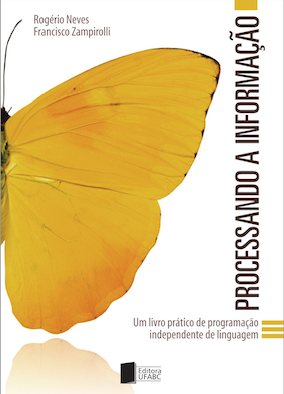
\includegraphics{"figs/Capa_Processando_Informacao.jpg"}

Este caderno (Notebook) é parte complementar \emph{online} do livro
\textbf{\href{https://editora.ufabc.edu.br/matematica-e-ciencias-da-computacao/58-processando-a-informacao}{Processando
a Informação}: um livro prático de programação independente de
linguagem}, que deve ser consultado no caso de dúvidas sobre os temas
apresentados.

\begin{quote}
Este conteúdo pode ser copiado e alterado livremente e foi inspirado
nesse livro.
\end{quote}

\begin{quote}
O conteúdo deste capítulo foi inspirado em: * Cap. 7: Conceitos de
programação orientada a objetos do livro anterior * Notas de aula de
professores da UFABC, em especial, dos professores Luiz Rozante e Wagner
Botelho.
\end{quote}

    \hypertarget{sumuxe1rio}{%
\subsection{Sumário}\label{sumuxe1rio}}

\begin{itemize}
\tightlist
\item
  Revisão do capítulo anterior
\item
  Introdução
\item
  Paradigma Estruturado
\item
  Paradigma Orientado a Objetos
\item
  Tipos de dados
\item
  Arquivos
\item
  Revisão deste capítulo
\item
  Exercícios
\end{itemize}

    \hypertarget{revisuxe3o-do-capuxedtulo-anterior-matriz}{%
\subsection{Revisão do capítulo anterior
(Matriz)}\label{revisuxe3o-do-capuxedtulo-anterior-matriz}}

    \begin{itemize}
\tightlist
\item
  Introdução
\item
  Instanciando matrizes
\item
  Acessando elementos de uma matriz
\item
  Formas de percorrer uma matriz
\item
  Aplicações usando matrizes
\item
  Exercícios
\end{itemize}

    \hypertarget{introduuxe7uxe3o}{%
\subsection{Introdução}\label{introduuxe7uxe3o}}

    \begin{itemize}
\tightlist
\item
  Este capítulo introduz alguns conceitos usados em:

  \begin{itemize}
  \tightlist
  \item
    Programação Estruturada,
  \item
    Programação Orientada a Objetos (POO) e
  \item
    Engenharia de Software (ES).
  \end{itemize}
\item
  Esses conceitos serão úteis em estudos futuros.
\item
  Não é o propósito deste capítulo cobrir completamente estes temas, mas
  sim proporcionar um ponto de partida para o estudo avançados em
  programação.
\item
  Além de introduzir processos para desenvolver códigos envolvendo
  equipes e utilizando princípios da Engenharia de Software.
\end{itemize}

    \hypertarget{paradigma-estruturado}{%
\subsection{Paradigma Estruturado}\label{paradigma-estruturado}}

    \begin{itemize}
\item
  Uns dos primeiros estilos (ou paradigma) para estruturar um Software é
  chamado de \textbf{Programação Estruturada}.
\item
  Neste paradigma estruturado, o programador define \textbf{Tabelas} (ou
  \textbf{Registros} ou também chamadas \textbf{Entidades}), onde se
  podem armazenar variáveis de vários tipos de dados,

  \begin{itemize}
  \tightlist
  \item
    diferentemente dos vetores e matrizes vistos nos capítulos anterios,
    onde todos os dados devem ser de um mesmo tipo de dado (exceto as
    listas em Python).
  \end{itemize}
\item
  Por exemplo, é possível definir uma tabela para armazenar as
  informações de um aluno num contexto de um sistema acadêmico, chamada
  \textbf{Aluno}.
\item
  Esta tabela \textbf{Aluno}, na verdade, pode ser considera um novo
  tipo de dados e é possível, por exemplo, ``instanciar'' uma variável
  (ou registro), como \emph{Julia} do tipo \textbf{Aluno}.
\item
  Como atributos da tabela \textbf{Aluno}, é possível ter \emph{nome},
  \emph{matrícula}, \emph{data de nascimento}, \emph{ano de ingresso},
  etc.
\item
  Observe que na tabela \textbf{Aluno} é importante também ter
  informação de curso e de disciplinas já cursadas.
\item
  Estas informações podem ser ``instâncias'' de outras tabelas, como
  \textbf{Curso} e \textbf{Disciplina}, com seus respectivos atributos
  apropriados.
\item
  Em Banco de Dados estas ``instâncias'' são possíveis através de um
  atributo representando a chave (estrangeira) de outra tabela.
\item
  Além disso, cada tabela possui um atributo (chamado chave primária)
  que identifica o registro, por exemplo, Julia, que pode estar
  armazenada num registro de número 33.
\item
  Resumindo, as \textbf{estrutura} definidas pelo programador podem
  armazenar em tempo de execução as \textbf{tabelas} definidas em Bancos
  de Dados (com informações armazenadas em disco).
\end{itemize}

    \hypertarget{diagrama-entidade-relacionamento}{%
\subsection{Diagrama Entidade
Relacionamento}\label{diagrama-entidade-relacionamento}}

    \begin{itemize}
\item
  Para poder visualizar melhor esta relação entre as tabelas
  \textbf{Aluno}, \textbf{Curso} e \textbf{Disciplina}, existe um modelo
  apropriado, chamado \textbf{Diagrama Entidade Relacionamento (DER)},
  como apresentado na figura abaixo.
\item
  Observe o relacionamento ``\textbf{Aluno} faz
  \textbf{Disciplina}(s)''.
\item
  Se for considerar um contexto onde um aluno está cursando uma
  disciplina, existe a necessidade de incluir uma nova tabela, chamada,
  por exemplo, \textbf{Turma}.
\item
  Assim, ``\textbf{Turma} possui \textbf{Aluno}(s)'' e
  ``\textbf{Disciplina} possui Turma(s)''.
\end{itemize}

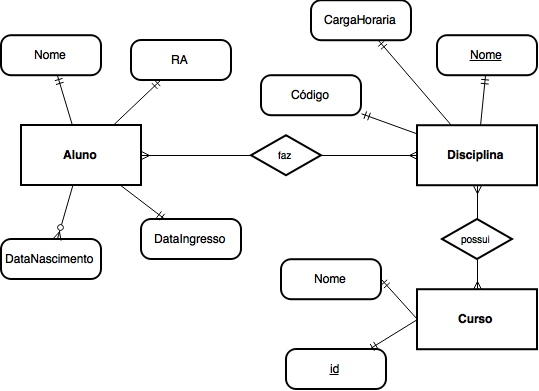
\includegraphics{"figs/image45.png"}

    \begin{figure}
\centering
\caption{image45.png}
\end{figure}

    \begin{itemize}
\item
  Desse modo, para um sistema acadêmico completo, é necessário criar
  várias tabelas e seus relacionamentos.
\item
  Todos esses dados das tabelas devem ser lidos (digitados) uma vez e
  armazenados em disco.
\item
  Senão, toda vez que esse sistema acadêmico for executado, todos os
  dados deverão ser lidos novamente.
\item
  Existem várias formas de guardar os dados de variáveis em disco:

  \begin{itemize}
  \tightlist
  \item
    arquivo texto,
  \item
    arquivo binário ou
  \item
    tabelas em um Sistema de Gerenciamento de Banco de Dados (SGBD),
    como Oracle, JDBC, SQL, PostgreSQL, etc.
  \end{itemize}
\item
  Nas disciplinas de Banco de Dados, o aluno aprende como criar essas
  tabelas em um SGBD e também como usá-las dentro de uma linguagem de
  programação.
\end{itemize}

    \begin{itemize}
\item
  Essa forma de organizar vários tipos de dados em tabelas chama-se
  \textbf{encapsulamento de dados}.
\item
  O grande desafio dos programadores e analistas de sistemas é definir
  corretamente essas tabelas e os seus relacionamentos. Os sistemas bem
  modelados são mais fáceis de realizar manutenções.
\item
  Além disso, os programadores devem criar estruturas, funções e
  procedimentos de forma bem organizada, por exemplo, usando vários
  arquivos organizados em pastas.
\item
  O paradigma estruturado não facilita completamente esta organização.
  Isso já não ocorre no paradigma orientado a objetos, resumido a
  seguir.
\end{itemize}

    \hypertarget{paradigma-orientado-a-objetos}{%
\subsection{Paradigma Orientado a
Objetos}\label{paradigma-orientado-a-objetos}}

    \begin{itemize}
\item
  Na programação estruturada não existe uma forma eficiente de organizar
  (encapsular) as funções específicas de uma tabela, como ocorre no
  encapsulamento dos dados, visto na programação estruturada.
\item
  Assim, surgiu a necessidade de criar um novo paradigma de programação,
  que é a \textbf{Programação Orientada a Objetos (POO)}, onde, além de
  encapsular os dados, é possível encapsular as funções ou métodos que
  os processam.
\item
  Na POO, tabela passou a se chamar \textbf{Classe}, e um registro de
  uma tabela passou a ser chamado de \textbf{instância} de uma classe,
  também chamado de \textbf{objeto}.
\item
  Como no exemplo anterior, para o sistema acadêmico, é possível criar a
  classe \textbf{Aluno} (que é um novo tipo de dados) e com ela
  instanciar uma variável \emph{Julia} da classe \textbf{Aluno}.
\end{itemize}

    O restante deste capítulo é complemetar ao livro
\textbf{\href{https://editora.ufabc.edu.br/matematica-e-ciencias-da-computacao/58-processando-a-informacao}{Processando
a Informação}: um livro prático de programação independente de
linguagem}, apresentando conceitos e exemplos de Programação
Estruturada.

    \hypertarget{tipos-de-dados}{%
\subsection{Tipos de dados}\label{tipos-de-dados}}

    \begin{itemize}
\item
  Os tipos de dados em C são:

  \begin{itemize}
  \tightlist
  \item
    \texttt{struct}
  \end{itemize}

\begin{verbatim}
struct MEU_TIPO{ 
 tipo1 nome1; 
 tipo2 nome2; 
 ... 
};
struct MEU_TIPO Entidade1, Entidade2; 
\end{verbatim}

  \begin{itemize}
  \tightlist
  \item
    Ou melhor, com \texttt{typedef} (utilizado para renomear um tipo de
    dado da própria linguagem ou definido pelo programador):
  \end{itemize}

\begin{verbatim}
typedef struct { 
tipo1 nome1; 
tipo2 nome2; 
... 
} MEU_TIPO;
MEU_TIPO Entidade1, Entidade2; 
\end{verbatim}

  \begin{itemize}
  \tightlist
  \item
    \texttt{union}
  \item
    \texttt{enum}
  \end{itemize}
\end{itemize}

    \hypertarget{exemplo-01---criar-um-registro-de-aluno}{%
\subsubsection{Exemplo 01 - Criar um registro de
Aluno}\label{exemplo-01---criar-um-registro-de-aluno}}

Exemplo para criar a \texttt{struct} \textbf{TAluno} contendo 4
atributos.

    \begin{tcolorbox}[breakable, size=fbox, boxrule=1pt, pad at break*=1mm,colback=cellbackground, colframe=cellborder]
\prompt{In}{incolor}{7}{\boxspacing}
\begin{Verbatim}[commandchars=\\\{\}]
\PY{o}{\PYZpc{}\PYZpc{}writefile} cap7ex01.c
\PY{c+c1}{\PYZsh{}include \PYZlt{}stdio.h\PYZgt{}}
\PY{c+c1}{\PYZsh{}include \PYZlt{}string.h\PYZgt{}}

\PY{n}{struct} \PY{n}{TAluno} \PY{p}{\PYZob{}}
  \PY{n}{char} \PY{n}{nome}\PY{p}{[}\PY{l+m+mi}{50}\PY{p}{]}\PY{p}{;}
  \PY{n+nb}{int} \PY{n}{idade}\PY{p}{;}
  \PY{n}{char} \PY{n}{rua}\PY{p}{[}\PY{l+m+mi}{50}\PY{p}{]}\PY{p}{;}
  \PY{n+nb}{int} \PY{n}{numero}\PY{p}{;}
\PY{p}{\PYZcb{}}\PY{p}{;}

\PY{n+nb}{int} \PY{n}{main}\PY{p}{(}\PY{p}{)} \PY{p}{\PYZob{}}
  \PY{n}{struct} \PY{n}{TAluno} \PY{n}{ana}\PY{p}{;} \PY{o}{/}\PY{o}{/} \PY{n}{instancia} \PY{n}{uma} \PY{n}{variável} \PY{n}{c} \PY{n}{do} \PY{n}{tipo} \PY{n}{TAluno}
  \PY{o}{/}\PY{o}{/} \PY{n}{ENTRADA} \PY{n}{DE} \PY{n}{DADOS}
  \PY{n}{strcpy}\PY{p}{(}\PY{n}{ana}\PY{o}{.}\PY{n}{nome}\PY{p}{,} \PY{l+s+s2}{\PYZdq{}}\PY{l+s+s2}{Ana Silva}\PY{l+s+s2}{\PYZdq{}}\PY{p}{)}\PY{p}{;}
  \PY{n}{ana}\PY{o}{.}\PY{n}{idade} \PY{o}{=} \PY{l+m+mi}{18}\PY{p}{;}
  \PY{n}{strcpy}\PY{p}{(}\PY{n}{ana}\PY{o}{.}\PY{n}{rua}\PY{p}{,} \PY{l+s+s2}{\PYZdq{}}\PY{l+s+s2}{Avenida Paulista}\PY{l+s+s2}{\PYZdq{}}\PY{p}{)}\PY{p}{;}
  \PY{n}{ana}\PY{o}{.}\PY{n}{numero} \PY{o}{=} \PY{l+m+mi}{1000}\PY{p}{;}

  \PY{o}{/}\PY{o}{/} \PY{n}{SAÍDA} \PY{n}{DE} \PY{n}{DADOS}
  \PY{n}{printf}\PY{p}{(}\PY{l+s+s2}{\PYZdq{}}\PY{l+s+s2}{nome: }\PY{l+s+si}{\PYZpc{}s}\PY{l+s+se}{\PYZbs{}n}\PY{l+s+s2}{idade: }\PY{l+s+si}{\PYZpc{}d}\PY{l+s+se}{\PYZbs{}n}\PY{l+s+s2}{\PYZdq{}}\PY{p}{,} \PY{n}{ana}\PY{o}{.}\PY{n}{nome}\PY{p}{,} \PY{n}{ana}\PY{o}{.}\PY{n}{idade}\PY{p}{)}\PY{p}{;}
  \PY{n}{printf}\PY{p}{(}\PY{l+s+s2}{\PYZdq{}}\PY{l+s+s2}{rua: }\PY{l+s+si}{\PYZpc{}s}\PY{l+s+se}{\PYZbs{}n}\PY{l+s+s2}{número: }\PY{l+s+si}{\PYZpc{}d}\PY{l+s+se}{\PYZbs{}n}\PY{l+s+s2}{\PYZdq{}}\PY{p}{,} \PY{n}{ana}\PY{o}{.}\PY{n}{rua}\PY{p}{,} \PY{n}{ana}\PY{o}{.}\PY{n}{numero}\PY{p}{)}\PY{p}{;}
  \PY{k}{return} \PY{l+m+mi}{0}\PY{p}{;}
\PY{p}{\PYZcb{}}
\end{Verbatim}
\end{tcolorbox}

    \begin{tcolorbox}[breakable, size=fbox, boxrule=1pt, pad at break*=1mm,colback=cellbackground, colframe=cellborder]
\prompt{In}{incolor}{8}{\boxspacing}
\begin{Verbatim}[commandchars=\\\{\}]
\PY{o}{\PYZpc{}\PYZpc{}}\PY{k}{shell}
gcc \PYZhy{}Wall \PYZhy{}std=c99 cap7ex01.c \PYZhy{}o output
./output
\end{Verbatim}
\end{tcolorbox}

    \hypertarget{exemplo-02---criar-um-registro-de-aluno-com-scanf}{%
\subsubsection{\texorpdfstring{Exemplo 02 - Criar um registro de Aluno,
com
\texttt{scanf}}{Exemplo 02 - Criar um registro de Aluno, com scanf}}\label{exemplo-02---criar-um-registro-de-aluno-com-scanf}}

Exemplo para criar a \texttt{struct} \textbf{TAluno} contendo 4
atributos lidos do teclado com \texttt{scanf}.

    \begin{tcolorbox}[breakable, size=fbox, boxrule=1pt, pad at break*=1mm,colback=cellbackground, colframe=cellborder]
\prompt{In}{incolor}{3}{\boxspacing}
\begin{Verbatim}[commandchars=\\\{\}]
\PY{o}{\PYZpc{}\PYZpc{}writefile} cap7ex02.c
\PY{c+c1}{\PYZsh{}include \PYZlt{}stdio.h\PYZgt{}}
\PY{c+c1}{\PYZsh{}include \PYZlt{}string.h\PYZgt{}}

\PY{n}{struct} \PY{n}{TAluno} \PY{p}{\PYZob{}}
  \PY{n}{char} \PY{n}{nome}\PY{p}{[}\PY{l+m+mi}{50}\PY{p}{]}\PY{p}{;}
  \PY{n+nb}{int} \PY{n}{idade}\PY{p}{;}
  \PY{n}{char} \PY{n}{rua}\PY{p}{[}\PY{l+m+mi}{50}\PY{p}{]}\PY{p}{;}
  \PY{n+nb}{int} \PY{n}{numero}\PY{p}{;}
\PY{p}{\PYZcb{}}\PY{p}{;}

\PY{n+nb}{int} \PY{n}{main}\PY{p}{(}\PY{p}{)} \PY{p}{\PYZob{}}
  \PY{n}{struct} \PY{n}{TAluno} \PY{n}{Alunos}\PY{p}{[}\PY{l+m+mi}{2}\PY{p}{]}\PY{p}{;} \PY{o}{/}\PY{o}{/} \PY{n}{instancia} \PY{n}{uma} \PY{n}{vetor} \PY{n}{do} \PY{n}{tipo} \PY{n}{TAluno}
  \PY{o}{/}\PY{o}{/} \PY{n}{ENTRADA} \PY{n}{DE} \PY{n}{DADOS}
  \PY{k}{for} \PY{p}{(}\PY{n+nb}{int} \PY{n}{i} \PY{o}{=} \PY{l+m+mi}{0}\PY{p}{;} \PY{n}{i} \PY{o}{\PYZlt{}} \PY{l+m+mi}{2}\PY{p}{;} \PY{n}{i}\PY{o}{+}\PY{o}{+}\PY{p}{)} \PY{p}{\PYZob{}}
    \PY{n}{printf}\PY{p}{(}\PY{l+s+s2}{\PYZdq{}}\PY{l+s+s2}{Entre com os dados: nome, idade, rua, número:}\PY{l+s+se}{\PYZbs{}n}\PY{l+s+s2}{\PYZdq{}}\PY{p}{)}\PY{p}{;}
    \PY{n}{fflush}\PY{p}{(}\PY{n}{stdin}\PY{p}{)}\PY{p}{;}
    \PY{n}{fgets}\PY{p}{(}\PY{n}{Alunos}\PY{p}{[}\PY{n}{i}\PY{p}{]}\PY{o}{.}\PY{n}{nome}\PY{p}{,} \PY{l+m+mi}{50}\PY{p}{,} \PY{n}{stdin}\PY{p}{)}\PY{p}{;}
    \PY{n}{scanf}\PY{p}{(}\PY{l+s+s2}{\PYZdq{}}\PY{l+s+si}{\PYZpc{}d}\PY{l+s+s2}{\PYZdq{}}\PY{p}{,} \PY{o}{\PYZam{}}\PY{n}{Alunos}\PY{p}{[}\PY{n}{i}\PY{p}{]}\PY{o}{.}\PY{n}{idade}\PY{p}{)}\PY{p}{;}
    \PY{n}{fflush}\PY{p}{(}\PY{n}{stdin}\PY{p}{)}\PY{p}{;}
    \PY{n}{fgets}\PY{p}{(}\PY{n}{Alunos}\PY{p}{[}\PY{n}{i}\PY{p}{]}\PY{o}{.}\PY{n}{rua}\PY{p}{,} \PY{l+m+mi}{50}\PY{p}{,} \PY{n}{stdin}\PY{p}{)}\PY{p}{;}
    \PY{n}{scanf}\PY{p}{(}\PY{l+s+s2}{\PYZdq{}}\PY{l+s+si}{\PYZpc{}d}\PY{l+s+s2}{\PYZdq{}}\PY{p}{,} \PY{o}{\PYZam{}}\PY{n}{Alunos}\PY{p}{[}\PY{n}{i}\PY{p}{]}\PY{o}{.}\PY{n}{numero}\PY{p}{)}\PY{p}{;}
  \PY{p}{\PYZcb{}}
  \PY{o}{/}\PY{o}{/} \PY{n}{SAÍDA} \PY{n}{DE} \PY{n}{DADOS}
  \PY{k}{for} \PY{p}{(}\PY{n+nb}{int} \PY{n}{i} \PY{o}{=} \PY{l+m+mi}{0}\PY{p}{;} \PY{n}{i} \PY{o}{\PYZlt{}} \PY{l+m+mi}{2}\PY{p}{;} \PY{n}{i}\PY{o}{+}\PY{o}{+}\PY{p}{)} \PY{p}{\PYZob{}}
    \PY{n}{printf}\PY{p}{(}\PY{l+s+s2}{\PYZdq{}}\PY{l+s+s2}{nome: }\PY{l+s+si}{\PYZpc{}s}\PY{l+s+se}{\PYZbs{}n}\PY{l+s+s2}{idade: }\PY{l+s+si}{\PYZpc{}d}\PY{l+s+se}{\PYZbs{}n}\PY{l+s+s2}{\PYZdq{}}\PY{p}{,} \PY{n}{Alunos}\PY{p}{[}\PY{n}{i}\PY{p}{]}\PY{o}{.}\PY{n}{nome}\PY{p}{,} \PY{n}{Alunos}\PY{p}{[}\PY{n}{i}\PY{p}{]}\PY{o}{.}\PY{n}{idade}\PY{p}{)}\PY{p}{;}
    \PY{n}{printf}\PY{p}{(}\PY{l+s+s2}{\PYZdq{}}\PY{l+s+s2}{rua: }\PY{l+s+si}{\PYZpc{}s}\PY{l+s+se}{\PYZbs{}n}\PY{l+s+s2}{número: }\PY{l+s+si}{\PYZpc{}d}\PY{l+s+se}{\PYZbs{}n}\PY{l+s+s2}{\PYZdq{}}\PY{p}{,} \PY{n}{Alunos}\PY{p}{[}\PY{n}{i}\PY{p}{]}\PY{o}{.}\PY{n}{rua}\PY{p}{,} \PY{n}{Alunos}\PY{p}{[}\PY{n}{i}\PY{p}{]}\PY{o}{.}\PY{n}{numero}\PY{p}{)}\PY{p}{;}
  \PY{p}{\PYZcb{}}
  \PY{k}{return} \PY{l+m+mi}{0}\PY{p}{;}
\PY{p}{\PYZcb{}}
\end{Verbatim}
\end{tcolorbox}

    \begin{tcolorbox}[breakable, size=fbox, boxrule=1pt, pad at break*=1mm,colback=cellbackground, colframe=cellborder]
\prompt{In}{incolor}{ }{\boxspacing}
\begin{Verbatim}[commandchars=\\\{\}]
\PY{o}{\PYZpc{}\PYZpc{}}\PY{k}{shell}
gcc \PYZhy{}Wall \PYZhy{}std=c99 cap7ex02.c \PYZhy{}o output
./output
\end{Verbatim}
\end{tcolorbox}

    \hypertarget{exemplo-03---criar-um-registro-de-aluno-com-typedef}{%
\subsubsection{\texorpdfstring{Exemplo 03 - Criar um registro de Aluno,
com
\texttt{typedef}}{Exemplo 03 - Criar um registro de Aluno, com typedef}}\label{exemplo-03---criar-um-registro-de-aluno-com-typedef}}

Exemplo para criar a \texttt{struct} \textbf{TAluno} contendo 4
atributos lidos do teclado, renomeando com \texttt{typedef} para
\textbf{Aluno}.

    \begin{tcolorbox}[breakable, size=fbox, boxrule=1pt, pad at break*=1mm,colback=cellbackground, colframe=cellborder]
\prompt{In}{incolor}{10}{\boxspacing}
\begin{Verbatim}[commandchars=\\\{\}]
\PY{o}{\PYZpc{}\PYZpc{}writefile} cap7ex03.c
\PY{c+c1}{\PYZsh{}include \PYZlt{}stdio.h\PYZgt{}}
\PY{c+c1}{\PYZsh{}include \PYZlt{}string.h\PYZgt{}}

\PY{n}{struct} \PY{n}{TAluno} \PY{p}{\PYZob{}}
  \PY{n}{char} \PY{n}{nome}\PY{p}{[}\PY{l+m+mi}{50}\PY{p}{]}\PY{p}{;}
  \PY{n+nb}{int} \PY{n}{idade}\PY{p}{;}
  \PY{n}{char} \PY{n}{rua}\PY{p}{[}\PY{l+m+mi}{50}\PY{p}{]}\PY{p}{;}
  \PY{n+nb}{int} \PY{n}{numero}\PY{p}{;}
\PY{p}{\PYZcb{}}\PY{p}{;}

\PY{n}{typedef} \PY{n}{struct} \PY{n}{TAluno} \PY{n}{Aluno}\PY{p}{;}

\PY{n+nb}{int} \PY{n}{main}\PY{p}{(}\PY{p}{)} \PY{p}{\PYZob{}}
  \PY{o}{/}\PY{o}{/} \PY{n}{ENTRADA} \PY{n}{DE} \PY{n}{DADOS}
  \PY{n}{Aluno} \PY{n}{Ana} \PY{o}{=} \PY{p}{\PYZob{}} \PY{l+s+s2}{\PYZdq{}}\PY{l+s+s2}{Ana Silva}\PY{l+s+s2}{\PYZdq{}} \PY{p}{,} \PY{l+m+mi}{18}\PY{p}{,} \PY{l+s+s2}{\PYZdq{}}\PY{l+s+s2}{Avenida Paulista}\PY{l+s+s2}{\PYZdq{}} \PY{p}{,} \PY{l+m+mi}{1000} \PY{p}{\PYZcb{}}\PY{p}{;}

  \PY{o}{/}\PY{o}{/} \PY{n}{SAÍDA} \PY{n}{DE} \PY{n}{DADOS}
  \PY{n}{printf}\PY{p}{(}\PY{l+s+s2}{\PYZdq{}}\PY{l+s+si}{\PYZpc{}s}\PY{l+s+s2}{ }\PY{l+s+si}{\PYZpc{}d}\PY{l+s+s2}{ }\PY{l+s+si}{\PYZpc{}s}\PY{l+s+s2}{ }\PY{l+s+si}{\PYZpc{}d}\PY{l+s+s2}{\PYZdq{}}\PY{p}{,} \PY{n}{Ana}\PY{o}{.}\PY{n}{nome}\PY{p}{,} \PY{n}{Ana}\PY{o}{.}\PY{n}{idade}\PY{p}{,} \PY{n}{Ana}\PY{o}{.}\PY{n}{rua}\PY{p}{,} \PY{n}{Ana}\PY{o}{.}\PY{n}{numero}\PY{p}{)}\PY{p}{;}
  \PY{k}{return} \PY{l+m+mi}{0}\PY{p}{;}
\PY{p}{\PYZcb{}}
\end{Verbatim}
\end{tcolorbox}

    \begin{tcolorbox}[breakable, size=fbox, boxrule=1pt, pad at break*=1mm,colback=cellbackground, colframe=cellborder]
\prompt{In}{incolor}{11}{\boxspacing}
\begin{Verbatim}[commandchars=\\\{\}]
\PY{o}{\PYZpc{}\PYZpc{}}\PY{k}{shell}
gcc \PYZhy{}Wall \PYZhy{}std=c99 cap7ex03.c \PYZhy{}o output
./output
\end{Verbatim}
\end{tcolorbox}

    \hypertarget{exemplo-04---criar-um-registro-de-aluno-com-typedef-opuxe7uxe3o-2}{%
\subsubsection{\texorpdfstring{Exemplo 04 - Criar um registro de Aluno,
com \texttt{typedef}, opção
2}{Exemplo 04 - Criar um registro de Aluno, com typedef, opção 2}}\label{exemplo-04---criar-um-registro-de-aluno-com-typedef-opuxe7uxe3o-2}}

Exemplo para criar a \texttt{struct} \textbf{Aluno} de forma
simplificada, contendo 4 atributos.

    \begin{tcolorbox}[breakable, size=fbox, boxrule=1pt, pad at break*=1mm,colback=cellbackground, colframe=cellborder]
\prompt{In}{incolor}{18}{\boxspacing}
\begin{Verbatim}[commandchars=\\\{\}]
\PY{o}{\PYZpc{}\PYZpc{}writefile} cap7ex04.c
\PY{c+c1}{\PYZsh{}include \PYZlt{}stdio.h\PYZgt{}}
\PY{c+c1}{\PYZsh{}include \PYZlt{}string.h\PYZgt{}}

\PY{n}{typedef} \PY{n}{struct} \PY{n}{TAluno} \PY{p}{\PYZob{}}
  \PY{n}{char} \PY{n}{nome}\PY{p}{[}\PY{l+m+mi}{50}\PY{p}{]}\PY{p}{;}
  \PY{n+nb}{int} \PY{n}{idade}\PY{p}{;}
  \PY{n}{char} \PY{n}{rua}\PY{p}{[}\PY{l+m+mi}{50}\PY{p}{]}\PY{p}{;}
  \PY{n+nb}{int} \PY{n}{numero}\PY{p}{;}
\PY{p}{\PYZcb{}} \PY{n}{Aluno}\PY{p}{;}

\PY{n+nb}{int} \PY{n}{main}\PY{p}{(}\PY{p}{)} \PY{p}{\PYZob{}}
  \PY{o}{/}\PY{o}{/} \PY{n}{ENTRADA} \PY{n}{DE} \PY{n}{DADOS}
  \PY{n}{Aluno} \PY{n}{ana} \PY{o}{=} \PY{p}{\PYZob{}} \PY{l+s+s2}{\PYZdq{}}\PY{l+s+s2}{Ana Silva}\PY{l+s+s2}{\PYZdq{}} \PY{p}{,} \PY{l+m+mi}{18}\PY{p}{,} \PY{l+s+s2}{\PYZdq{}}\PY{l+s+s2}{Avenida Paulista}\PY{l+s+s2}{\PYZdq{}} \PY{p}{,} \PY{l+m+mi}{1000} \PY{p}{\PYZcb{}}\PY{p}{;}

  \PY{o}{/}\PY{o}{/} \PY{n}{SAÍDA} \PY{n}{DE} \PY{n}{DADOS}
  \PY{n}{printf}\PY{p}{(}\PY{l+s+s2}{\PYZdq{}}\PY{l+s+si}{\PYZpc{}s}\PY{l+s+s2}{ }\PY{l+s+si}{\PYZpc{}d}\PY{l+s+s2}{ }\PY{l+s+si}{\PYZpc{}s}\PY{l+s+s2}{ }\PY{l+s+si}{\PYZpc{}d}\PY{l+s+s2}{\PYZdq{}}\PY{p}{,} \PY{n}{ana}\PY{o}{.}\PY{n}{nome}\PY{p}{,} \PY{n}{ana}\PY{o}{.}\PY{n}{idade}\PY{p}{,} \PY{n}{ana}\PY{o}{.}\PY{n}{rua}\PY{p}{,} \PY{n}{ana}\PY{o}{.}\PY{n}{numero}\PY{p}{)}\PY{p}{;}
  \PY{k}{return} \PY{l+m+mi}{0}\PY{p}{;}
\PY{p}{\PYZcb{}}
\end{Verbatim}
\end{tcolorbox}

    \begin{tcolorbox}[breakable, size=fbox, boxrule=1pt, pad at break*=1mm,colback=cellbackground, colframe=cellborder]
\prompt{In}{incolor}{19}{\boxspacing}
\begin{Verbatim}[commandchars=\\\{\}]
\PY{o}{\PYZpc{}\PYZpc{}}\PY{k}{shell}
gcc \PYZhy{}Wall \PYZhy{}std=c99 cap7ex04.c \PYZhy{}o output
./output
\end{Verbatim}
\end{tcolorbox}

    \hypertarget{exemplo-05---criar-dois-registros}{%
\subsubsection{Exemplo 05 - Criar dois
registros}\label{exemplo-05---criar-dois-registros}}

Exemplo para criar a \texttt{struct} \textbf{Cliente} contendo 3
atributos, sendo um deles uma outra estrutura \textbf{Endereco}.

    \begin{tcolorbox}[breakable, size=fbox, boxrule=1pt, pad at break*=1mm,colback=cellbackground, colframe=cellborder]
\prompt{In}{incolor}{61}{\boxspacing}
\begin{Verbatim}[commandchars=\\\{\}]
\PY{o}{\PYZpc{}\PYZpc{}writefile} cap7ex05.c
\PY{c+c1}{\PYZsh{}include \PYZlt{}stdio.h\PYZgt{}}
\PY{c+c1}{\PYZsh{}include \PYZlt{}string.h\PYZgt{}}

\PY{n}{typedef} \PY{n}{struct} \PY{p}{\PYZob{}}
  \PY{n}{char} \PY{n}{rua}\PY{p}{[}\PY{l+m+mi}{50}\PY{p}{]}\PY{p}{;}
  \PY{n+nb}{int} \PY{n}{numero}\PY{p}{;}
\PY{p}{\PYZcb{}} \PY{n}{Endereco}\PY{p}{;}

\PY{n}{typedef} \PY{n}{struct} \PY{p}{\PYZob{}}
  \PY{n}{char} \PY{n}{nome}\PY{p}{[}\PY{l+m+mi}{50}\PY{p}{]}\PY{p}{;}
  \PY{n+nb}{int} \PY{n}{idade}\PY{p}{;}
  \PY{n}{Endereco} \PY{n}{end}\PY{p}{;}
\PY{p}{\PYZcb{}} \PY{n}{Cliente}\PY{p}{;}

\PY{n}{void} \PY{n}{leiaCliente}\PY{p}{(}\PY{n}{Cliente}\PY{o}{*} \PY{n}{cliente}\PY{p}{)} \PY{p}{\PYZob{}}
  \PY{n}{fflush}\PY{p}{(}\PY{n}{stdin}\PY{p}{)}\PY{p}{;}
  \PY{n}{printf}\PY{p}{(}\PY{l+s+s2}{\PYZdq{}}\PY{l+s+s2}{nome: }\PY{l+s+s2}{\PYZdq{}}\PY{p}{)}\PY{p}{;}
  \PY{n}{fgets}\PY{p}{(}\PY{p}{(}\PY{o}{*}\PY{n}{cliente}\PY{p}{)}\PY{o}{.}\PY{n}{nome}\PY{p}{,} \PY{l+m+mi}{50}\PY{p}{,} \PY{n}{stdin}\PY{p}{)}\PY{p}{;}
  \PY{n}{printf}\PY{p}{(}\PY{l+s+s2}{\PYZdq{}}\PY{l+s+s2}{idade: }\PY{l+s+s2}{\PYZdq{}}\PY{p}{)}\PY{p}{;}
  \PY{n}{scanf}\PY{p}{(}\PY{l+s+s2}{\PYZdq{}}\PY{l+s+si}{\PYZpc{}d}\PY{l+s+s2}{\PYZdq{}}\PY{p}{,} \PY{o}{\PYZam{}}\PY{p}{(}\PY{o}{*}\PY{n}{cliente}\PY{p}{)}\PY{o}{.}\PY{n}{idade}\PY{p}{)}\PY{p}{;}
  \PY{n}{fflush}\PY{p}{(}\PY{n}{stdin}\PY{p}{)}\PY{p}{;}
  \PY{n}{printf}\PY{p}{(}\PY{l+s+s2}{\PYZdq{}}\PY{l+s+s2}{rua: }\PY{l+s+s2}{\PYZdq{}}\PY{p}{)}\PY{p}{;}
  \PY{n}{fgets}\PY{p}{(}\PY{p}{(}\PY{o}{*}\PY{n}{cliente}\PY{p}{)}\PY{o}{.}\PY{n}{end}\PY{o}{.}\PY{n}{rua}\PY{p}{,} \PY{l+m+mi}{50}\PY{p}{,} \PY{n}{stdin}\PY{p}{)}\PY{p}{;}
  \PY{n}{printf}\PY{p}{(}\PY{l+s+s2}{\PYZdq{}}\PY{l+s+s2}{numero: }\PY{l+s+s2}{\PYZdq{}}\PY{p}{)}\PY{p}{;}
  \PY{n}{scanf}\PY{p}{(}\PY{l+s+s2}{\PYZdq{}}\PY{l+s+si}{\PYZpc{}d}\PY{l+s+s2}{\PYZdq{}}\PY{p}{,} \PY{o}{\PYZam{}}\PY{p}{(}\PY{o}{*}\PY{n}{cliente}\PY{p}{)}\PY{o}{.}\PY{n}{end}\PY{o}{.}\PY{n}{numero}\PY{p}{)}\PY{p}{;}
\PY{p}{\PYZcb{}}

\PY{n}{void} \PY{n}{escrevaCliente}\PY{p}{(}\PY{n}{Cliente} \PY{n}{cliente}\PY{p}{)} \PY{p}{\PYZob{}}
  \PY{n}{printf}\PY{p}{(}\PY{l+s+s2}{\PYZdq{}}\PY{l+s+s2}{nome: }\PY{l+s+si}{\PYZpc{}s}\PY{l+s+se}{\PYZbs{}n}\PY{l+s+s2}{idade: }\PY{l+s+si}{\PYZpc{}d}\PY{l+s+se}{\PYZbs{}n}\PY{l+s+s2}{\PYZdq{}}\PY{p}{,} \PY{n}{cliente}\PY{o}{.}\PY{n}{nome}\PY{p}{,} \PY{n}{cliente}\PY{o}{.}\PY{n}{idade}\PY{p}{)}\PY{p}{;}
  \PY{n}{printf}\PY{p}{(}\PY{l+s+s2}{\PYZdq{}}\PY{l+s+s2}{rua: }\PY{l+s+si}{\PYZpc{}s}\PY{l+s+se}{\PYZbs{}n}\PY{l+s+s2}{numero: }\PY{l+s+si}{\PYZpc{}d}\PY{l+s+se}{\PYZbs{}n}\PY{l+s+s2}{\PYZdq{}}\PY{p}{,} \PY{n}{cliente}\PY{o}{.}\PY{n}{end}\PY{o}{.}\PY{n}{rua}\PY{p}{,} \PY{n}{cliente}\PY{o}{.}\PY{n}{end}\PY{o}{.}\PY{n}{numero}\PY{p}{)}\PY{p}{;}
\PY{p}{\PYZcb{}}

\PY{n+nb}{int} \PY{n}{main}\PY{p}{(}\PY{p}{)} \PY{p}{\PYZob{}}
  \PY{n}{Cliente} \PY{n}{clientes}\PY{p}{[}\PY{l+m+mi}{2}\PY{p}{]}\PY{p}{;}
  \PY{o}{/}\PY{o}{/} \PY{n}{ENTRADA} \PY{n}{DE} \PY{n}{DADOS}
  \PY{k}{for} \PY{p}{(}\PY{n+nb}{int} \PY{n}{i} \PY{o}{=} \PY{l+m+mi}{0}\PY{p}{;} \PY{n}{i} \PY{o}{\PYZlt{}} \PY{l+m+mi}{2}\PY{p}{;} \PY{n}{i}\PY{o}{+}\PY{o}{+}\PY{p}{)} \PY{p}{\PYZob{}}
    \PY{n}{printf}\PY{p}{(}\PY{l+s+s2}{\PYZdq{}}\PY{l+s+s2}{Cadastrar dados do cliente }\PY{l+s+si}{\PYZpc{}d}\PY{l+s+se}{\PYZbs{}n}\PY{l+s+s2}{\PYZdq{}}\PY{p}{,} \PY{n}{i} \PY{o}{+} \PY{l+m+mi}{1}\PY{p}{)}\PY{p}{;}
    \PY{n}{leiaCliente}\PY{p}{(}\PY{o}{\PYZam{}}\PY{n}{clientes}\PY{p}{[}\PY{n}{i}\PY{p}{]}\PY{p}{)}\PY{p}{;}
  \PY{p}{\PYZcb{}}

  \PY{o}{/}\PY{o}{/} \PY{n}{SAÍDA} \PY{n}{DE} \PY{n}{DADOS}
  \PY{k}{for} \PY{p}{(}\PY{n+nb}{int} \PY{n}{i} \PY{o}{=} \PY{l+m+mi}{0}\PY{p}{;} \PY{n}{i} \PY{o}{\PYZlt{}} \PY{l+m+mi}{2}\PY{p}{;} \PY{n}{i}\PY{o}{+}\PY{o}{+}\PY{p}{)} \PY{p}{\PYZob{}}
    \PY{n}{printf}\PY{p}{(}\PY{l+s+s2}{\PYZdq{}}\PY{l+s+s2}{Imprimir dados do cliente }\PY{l+s+si}{\PYZpc{}d}\PY{l+s+se}{\PYZbs{}n}\PY{l+s+s2}{\PYZdq{}}\PY{p}{,} \PY{n}{i} \PY{o}{+} \PY{l+m+mi}{1}\PY{p}{)}\PY{p}{;}
    \PY{n}{escrevaCliente}\PY{p}{(}\PY{n}{clientes}\PY{p}{[}\PY{n}{i}\PY{p}{]}\PY{p}{)}\PY{p}{;}
  \PY{p}{\PYZcb{}}
  \PY{k}{return} \PY{l+m+mi}{0}\PY{p}{;}
\PY{p}{\PYZcb{}}
\end{Verbatim}
\end{tcolorbox}

    \begin{tcolorbox}[breakable, size=fbox, boxrule=1pt, pad at break*=1mm,colback=cellbackground, colframe=cellborder]
\prompt{In}{incolor}{ }{\boxspacing}
\begin{Verbatim}[commandchars=\\\{\}]
\PY{o}{\PYZpc{}\PYZpc{}}\PY{k}{shell}
gcc \PYZhy{}Wall \PYZhy{}std=c99 cap7ex05.c \PYZhy{}o output
./output
\end{Verbatim}
\end{tcolorbox}

    \hypertarget{exemplo-06---criar-dois-registros-usando-biblioteca}{%
\subsubsection{Exemplo 06 - Criar dois registros usando
biblioteca}\label{exemplo-06---criar-dois-registros-usando-biblioteca}}

Exemplo para criar a \texttt{struct} \textbf{Cliente} contendo 3
atributos, sendo um deles uma outra estrutura \textbf{Endereco},
organizados em uma biblioteca.

    \begin{tcolorbox}[breakable, size=fbox, boxrule=1pt, pad at break*=1mm,colback=cellbackground, colframe=cellborder]
\prompt{In}{incolor}{57}{\boxspacing}
\begin{Verbatim}[commandchars=\\\{\}]
\PY{o}{\PYZpc{}\PYZpc{}writefile} cap7ex06.c
\PY{c+c1}{\PYZsh{}include \PYZdq{}myBiblioteca.h\PYZdq{}}

\PY{n+nb}{int} \PY{n}{main}\PY{p}{(}\PY{p}{)} \PY{p}{\PYZob{}}
  \PY{n}{Cliente} \PY{n}{clientes}\PY{p}{[}\PY{l+m+mi}{2}\PY{p}{]}\PY{p}{;}
  \PY{o}{/}\PY{o}{/} \PY{n}{ENTRADA} \PY{n}{DE} \PY{n}{DADOS}
  \PY{k}{for} \PY{p}{(}\PY{n+nb}{int} \PY{n}{i} \PY{o}{=} \PY{l+m+mi}{0}\PY{p}{;} \PY{n}{i} \PY{o}{\PYZlt{}} \PY{l+m+mi}{2}\PY{p}{;} \PY{n}{i}\PY{o}{+}\PY{o}{+}\PY{p}{)} \PY{p}{\PYZob{}}
    \PY{n}{printf}\PY{p}{(}\PY{l+s+s2}{\PYZdq{}}\PY{l+s+s2}{Cadastrar dados do cliente }\PY{l+s+si}{\PYZpc{}d}\PY{l+s+se}{\PYZbs{}n}\PY{l+s+s2}{\PYZdq{}}\PY{p}{,} \PY{n}{i} \PY{o}{+} \PY{l+m+mi}{1}\PY{p}{)}\PY{p}{;}
    \PY{n}{leiaCliente}\PY{p}{(}\PY{o}{\PYZam{}}\PY{n}{clientes}\PY{p}{[}\PY{n}{i}\PY{p}{]}\PY{p}{)}\PY{p}{;}
  \PY{p}{\PYZcb{}}

  \PY{o}{/}\PY{o}{/} \PY{n}{SAÍDA} \PY{n}{DE} \PY{n}{DADOS}
  \PY{k}{for} \PY{p}{(}\PY{n+nb}{int} \PY{n}{i} \PY{o}{=} \PY{l+m+mi}{0}\PY{p}{;} \PY{n}{i} \PY{o}{\PYZlt{}} \PY{l+m+mi}{2}\PY{p}{;} \PY{n}{i}\PY{o}{+}\PY{o}{+}\PY{p}{)} \PY{p}{\PYZob{}}
    \PY{n}{printf}\PY{p}{(}\PY{l+s+s2}{\PYZdq{}}\PY{l+s+s2}{Imprimir dados do cliente }\PY{l+s+si}{\PYZpc{}d}\PY{l+s+se}{\PYZbs{}n}\PY{l+s+s2}{\PYZdq{}}\PY{p}{,} \PY{n}{i} \PY{o}{+} \PY{l+m+mi}{1}\PY{p}{)}\PY{p}{;}
    \PY{n}{escrevaCliente}\PY{p}{(}\PY{n}{clientes}\PY{p}{[}\PY{n}{i}\PY{p}{]}\PY{p}{)}\PY{p}{;}
  \PY{p}{\PYZcb{}}
  \PY{k}{return} \PY{l+m+mi}{0}\PY{p}{;}
\PY{p}{\PYZcb{}}
\end{Verbatim}
\end{tcolorbox}

    \begin{tcolorbox}[breakable, size=fbox, boxrule=1pt, pad at break*=1mm,colback=cellbackground, colframe=cellborder]
\prompt{In}{incolor}{58}{\boxspacing}
\begin{Verbatim}[commandchars=\\\{\}]
\PY{o}{\PYZpc{}\PYZpc{}writefile} myBiblioteca.h
\PY{c+c1}{\PYZsh{}include \PYZlt{}stdio.h\PYZgt{}}
\PY{c+c1}{\PYZsh{}include \PYZlt{}string.h\PYZgt{}}
\PY{c+c1}{\PYZsh{}include \PYZlt{}stdlib.h\PYZgt{}}

\PY{n}{typedef} \PY{n}{struct} \PY{p}{\PYZob{}}
  \PY{n}{char} \PY{n}{rua}\PY{p}{[}\PY{l+m+mi}{50}\PY{p}{]}\PY{p}{;}
  \PY{n+nb}{int} \PY{n}{numero}\PY{p}{;}
\PY{p}{\PYZcb{}} \PY{n}{Endereco}\PY{p}{;}

\PY{n}{typedef} \PY{n}{struct} \PY{p}{\PYZob{}}
  \PY{n}{char} \PY{n}{nome}\PY{p}{[}\PY{l+m+mi}{50}\PY{p}{]}\PY{p}{;}
  \PY{n+nb}{int} \PY{n}{idade}\PY{p}{;}
  \PY{n}{Endereco} \PY{n}{end}\PY{p}{;}
\PY{p}{\PYZcb{}} \PY{n}{Cliente}\PY{p}{;}

\PY{n}{void} \PY{n}{leiaCliente}\PY{p}{(}\PY{n}{Cliente}\PY{o}{*} \PY{n}{cliente}\PY{p}{)}\PY{p}{;}
\PY{n}{void} \PY{n}{escrevaCliente}\PY{p}{(}\PY{n}{Cliente} \PY{n}{cliente}\PY{p}{)}\PY{p}{;}
\end{Verbatim}
\end{tcolorbox}

    \begin{tcolorbox}[breakable, size=fbox, boxrule=1pt, pad at break*=1mm,colback=cellbackground, colframe=cellborder]
\prompt{In}{incolor}{59}{\boxspacing}
\begin{Verbatim}[commandchars=\\\{\}]
\PY{o}{\PYZpc{}\PYZpc{}writefile} myBiblioteca.c
\PY{c+c1}{\PYZsh{}include \PYZdq{}myBiblioteca.h\PYZdq{}}

\PY{n}{void} \PY{n}{escrevaCliente}\PY{p}{(}\PY{n}{Cliente} \PY{n}{cliente}\PY{p}{)} \PY{p}{\PYZob{}}
  \PY{n}{printf}\PY{p}{(}\PY{l+s+s2}{\PYZdq{}}\PY{l+s+s2}{nome: }\PY{l+s+si}{\PYZpc{}s}\PY{l+s+se}{\PYZbs{}n}\PY{l+s+s2}{idade: }\PY{l+s+si}{\PYZpc{}d}\PY{l+s+se}{\PYZbs{}n}\PY{l+s+s2}{\PYZdq{}}\PY{p}{,} \PY{n}{cliente}\PY{o}{.}\PY{n}{nome}\PY{p}{,} \PY{n}{cliente}\PY{o}{.}\PY{n}{idade}\PY{p}{)}\PY{p}{;}
  \PY{n}{printf}\PY{p}{(}\PY{l+s+s2}{\PYZdq{}}\PY{l+s+s2}{rua: }\PY{l+s+si}{\PYZpc{}s}\PY{l+s+se}{\PYZbs{}n}\PY{l+s+s2}{número: }\PY{l+s+si}{\PYZpc{}d}\PY{l+s+se}{\PYZbs{}n}\PY{l+s+s2}{\PYZdq{}}\PY{p}{,} \PY{n}{cliente}\PY{o}{.}\PY{n}{end}\PY{o}{.}\PY{n}{rua}\PY{p}{,} \PY{n}{cliente}\PY{o}{.}\PY{n}{end}\PY{o}{.}\PY{n}{numero}\PY{p}{)}\PY{p}{;}
\PY{p}{\PYZcb{}}

\PY{o}{/}\PY{o}{/} \PY{n}{leia} \PY{n}{um} \PY{n}{cliente} \PY{n}{a} \PY{n}{partir} \PY{n}{do} \PY{n}{teclado}
\PY{o}{/}\PY{o}{/} \PY{n}{nome}\PY{p}{,} \PY{n}{idade}\PY{p}{,} \PY{n}{rua}\PY{p}{,} \PY{n}{numero}
\PY{n}{void} \PY{n}{leiaCliente}\PY{p}{(}\PY{n}{Cliente}\PY{o}{*} \PY{n}{cliente}\PY{p}{)} \PY{p}{\PYZob{}}
  \PY{n}{fflush}\PY{p}{(}\PY{n}{stdin}\PY{p}{)}\PY{p}{;}
  \PY{n}{printf}\PY{p}{(}\PY{l+s+s2}{\PYZdq{}}\PY{l+s+s2}{nome: }\PY{l+s+s2}{\PYZdq{}}\PY{p}{)}\PY{p}{;}
  \PY{n}{fgets}\PY{p}{(}\PY{p}{(}\PY{o}{*}\PY{n}{cliente}\PY{p}{)}\PY{o}{.}\PY{n}{nome}\PY{p}{,} \PY{l+m+mi}{50}\PY{p}{,} \PY{n}{stdin}\PY{p}{)}\PY{p}{;}
  \PY{n}{printf}\PY{p}{(}\PY{l+s+s2}{\PYZdq{}}\PY{l+s+s2}{idade: }\PY{l+s+s2}{\PYZdq{}}\PY{p}{)}\PY{p}{;}
  \PY{n}{scanf}\PY{p}{(}\PY{l+s+s2}{\PYZdq{}}\PY{l+s+si}{\PYZpc{}d}\PY{l+s+s2}{\PYZdq{}}\PY{p}{,} \PY{o}{\PYZam{}}\PY{p}{(}\PY{o}{*}\PY{n}{cliente}\PY{p}{)}\PY{o}{.}\PY{n}{idade}\PY{p}{)}\PY{p}{;}
  \PY{n}{fflush}\PY{p}{(}\PY{n}{stdin}\PY{p}{)}\PY{p}{;}
  \PY{n}{printf}\PY{p}{(}\PY{l+s+s2}{\PYZdq{}}\PY{l+s+s2}{rua: }\PY{l+s+s2}{\PYZdq{}}\PY{p}{)}\PY{p}{;}
  \PY{n}{fgets}\PY{p}{(}\PY{p}{(}\PY{o}{*}\PY{n}{cliente}\PY{p}{)}\PY{o}{.}\PY{n}{end}\PY{o}{.}\PY{n}{rua}\PY{p}{,} \PY{l+m+mi}{50}\PY{p}{,} \PY{n}{stdin}\PY{p}{)}\PY{p}{;}
  \PY{n}{printf}\PY{p}{(}\PY{l+s+s2}{\PYZdq{}}\PY{l+s+s2}{numero: }\PY{l+s+s2}{\PYZdq{}}\PY{p}{)}\PY{p}{;}
  \PY{n}{scanf}\PY{p}{(}\PY{l+s+s2}{\PYZdq{}}\PY{l+s+si}{\PYZpc{}d}\PY{l+s+s2}{\PYZdq{}}\PY{p}{,} \PY{o}{\PYZam{}}\PY{p}{(}\PY{o}{*}\PY{n}{cliente}\PY{p}{)}\PY{o}{.}\PY{n}{end}\PY{o}{.}\PY{n}{numero}\PY{p}{)}\PY{p}{;}
\PY{p}{\PYZcb{}}
\end{Verbatim}
\end{tcolorbox}

    \begin{tcolorbox}[breakable, size=fbox, boxrule=1pt, pad at break*=1mm,colback=cellbackground, colframe=cellborder]
\prompt{In}{incolor}{ }{\boxspacing}
\begin{Verbatim}[commandchars=\\\{\}]
\PY{o}{\PYZpc{}\PYZpc{}}\PY{k}{shell}
gcc \PYZhy{}Wall \PYZhy{}std=c99 cap7ex06.c myBiblioteca.c \PYZhy{}o output
./output
\end{Verbatim}
\end{tcolorbox}

    \hypertarget{arquivos}{%
\subsection{Arquivos}\label{arquivos}}

Os arquivos armazenados em disco são considerados como uma sequência de
caracteres e podem ser acessados em memória através de um ponteiro para
o primeiro caracter do arquivo (texto ou binário), como segue:

\begin{verbatim}
FILE *fp;
fp = fopen("nomeArquivo.txt", "modo"); // modo é definido a seguir
\end{verbatim}

Seguem as principais funções para manipular arquivos da biblioteca
\texttt{stdio.h}:

\begin{longtable}[]{@{}cl@{}}
\toprule
Função & Descrição\tabularnewline
\midrule
\endhead
\texttt{fopen()} & Abre arquivo\tabularnewline
\texttt{fclose()} & Fecha arquivo\tabularnewline
\texttt{putc()} & Escreve um caracter no arquivo\tabularnewline
\texttt{fputc()} & Igual \texttt{putc()}\tabularnewline
\texttt{getc()} & Lê um caracter do arquivo\tabularnewline
\texttt{fgetc()} & Igual \texttt{getc()}\tabularnewline
\texttt{fseek()} & Posiciona o arquivo em um determinado
byte\tabularnewline
\texttt{fprintf()} & Semelhante ao \texttt{printf()}, mas para
arquivo\tabularnewline
\texttt{fscanf()} & Semelhante ao \texttt{scanf()}, mas para
arquivo\tabularnewline
\texttt{feof()} & Verifica final de arquivo\tabularnewline
\texttt{ferror()} & Verifica se ocorreu erro\tabularnewline
\texttt{rewind()} & Posiciona o ponteiro para o início do
arquivo\tabularnewline
\texttt{remove()} & Apaga arquivo\tabularnewline
\texttt{fflush()} & Descarrega o \emph{buffer} do arquivo\tabularnewline
\texttt{fgets()} & Obtém uma string do arquivo\tabularnewline
\texttt{fread()} & Lê um bloco de dados do arquivo\tabularnewline
\texttt{fwrite()} & Escreve um bloco de dados no arquivo\tabularnewline
\texttt{ftell()} & Retorna a posição do ponteiro\tabularnewline
\bottomrule
\end{longtable}

    \begin{longtable}[]{@{}ccc@{}}
\toprule
\textbf{Modo} & \textbf{Arquivo} & \textbf{Função}\tabularnewline
\midrule
\endhead
r & Texto & Leitura\tabularnewline
w & Texto & Escrita em arquivo novo\tabularnewline
a & Texto & Escrita em arquivo existente\tabularnewline
r+ & Texto & Leitura/Escrita\tabularnewline
w+ & Texto & Leitura/Escrita\tabularnewline
a+ & Texto & Leitura/Escrita\tabularnewline
rb & Binário & Leitura\tabularnewline
wb & Binário & Escrita\tabularnewline
ab & Binário & Escrita\tabularnewline
r+b & Binário & Leitura/Escrita\tabularnewline
w+b & Binário & Leitura/Escrita\tabularnewline
a+b & Binário & Leitura/Escrita\tabularnewline
\bottomrule
\end{longtable}

    \hypertarget{exemplo-07---criar-arquivo}{%
\subsubsection{Exemplo 07 - Criar
Arquivo}\label{exemplo-07---criar-arquivo}}

Exemplo para criar um arquivo texto.

    \begin{tcolorbox}[breakable, size=fbox, boxrule=1pt, pad at break*=1mm,colback=cellbackground, colframe=cellborder]
\prompt{In}{incolor}{41}{\boxspacing}
\begin{Verbatim}[commandchars=\\\{\}]
\PY{o}{\PYZpc{}\PYZpc{}writefile} cap7ex07.c
\PY{c+c1}{\PYZsh{}include \PYZlt{}stdio.h\PYZgt{}}

\PY{n+nb}{int} \PY{n}{main}\PY{p}{(}\PY{p}{)} \PY{p}{\PYZob{}}
  \PY{n}{char}\PY{o}{*} \PY{n}{filename} \PY{o}{=} \PY{l+s+s2}{\PYZdq{}}\PY{l+s+s2}{teste.txt}\PY{l+s+s2}{\PYZdq{}}\PY{p}{;}
  \PY{n}{FILE}\PY{o}{*} \PY{n}{file}\PY{p}{;}

  \PY{n}{file} \PY{o}{=} \PY{n}{fopen}\PY{p}{(}\PY{n}{filename}\PY{p}{,} \PY{l+s+s2}{\PYZdq{}}\PY{l+s+s2}{w}\PY{l+s+s2}{\PYZdq{}}\PY{p}{)}\PY{p}{;} \PY{o}{/}\PY{o}{/} \PY{n}{Cria} \PY{n}{arquivo} \PY{n}{para} \PY{n}{escrita}
  \PY{k}{if} \PY{p}{(}\PY{n}{file} \PY{o}{==} \PY{n}{NULL}\PY{p}{)} \PY{p}{\PYZob{}}
    \PY{n}{printf}\PY{p}{(}\PY{l+s+s2}{\PYZdq{}}\PY{l+s+s2}{Erro ao abrir o arquivo: }\PY{l+s+si}{\PYZpc{}s}\PY{l+s+se}{\PYZbs{}n}\PY{l+s+s2}{\PYZdq{}}\PY{p}{,} \PY{n}{filename}\PY{p}{)}\PY{p}{;}
    \PY{k}{return} \PY{o}{\PYZhy{}}\PY{l+m+mi}{1}\PY{p}{;}
  \PY{p}{\PYZcb{}}

  \PY{o}{/}\PY{o}{/} \PY{n}{SAÍDA} \PY{n}{DE} \PY{n}{DADOS}
  \PY{k}{for} \PY{p}{(}\PY{n+nb}{int} \PY{n}{i} \PY{o}{=} \PY{l+m+mi}{0}\PY{p}{;} \PY{n}{i} \PY{o}{\PYZlt{}} \PY{l+m+mi}{10}\PY{p}{;} \PY{n}{i}\PY{o}{+}\PY{o}{+}\PY{p}{)}
    \PY{n}{fprintf}\PY{p}{(}\PY{n}{file}\PY{p}{,} \PY{l+s+s2}{\PYZdq{}}\PY{l+s+s2}{Linha }\PY{l+s+si}{\PYZpc{}02d}\PY{l+s+se}{\PYZbs{}n}\PY{l+s+s2}{\PYZdq{}}\PY{p}{,} \PY{n}{i} \PY{o}{+} \PY{l+m+mi}{1}\PY{p}{)}\PY{p}{;} \PY{o}{/}\PY{o}{/} \PY{n}{Escrever} \PY{n}{algo} \PY{n}{no} \PY{n}{arquivo}

  \PY{n}{fclose}\PY{p}{(}\PY{n}{file}\PY{p}{)}\PY{p}{;} \PY{o}{/}\PY{o}{/} \PY{n}{fecha} \PY{n}{arquivo}
  \PY{k}{return} \PY{l+m+mi}{0}\PY{p}{;}
\PY{p}{\PYZcb{}}
\end{Verbatim}
\end{tcolorbox}

    \begin{tcolorbox}[breakable, size=fbox, boxrule=1pt, pad at break*=1mm,colback=cellbackground, colframe=cellborder]
\prompt{In}{incolor}{ }{\boxspacing}
\begin{Verbatim}[commandchars=\\\{\}]
\PY{o}{\PYZpc{}\PYZpc{}}\PY{k}{shell}
gcc \PYZhy{}Wall \PYZhy{}std=c99 cap7ex07.c \PYZhy{}o output
./output
cat teste.txt
\end{Verbatim}
\end{tcolorbox}

    \hypertarget{exemplo-08---ler-arquivo}{%
\subsubsection{Exemplo 08 - Ler
arquivo}\label{exemplo-08---ler-arquivo}}

Exemplo para ler um arquivo texto.

    \begin{tcolorbox}[breakable, size=fbox, boxrule=1pt, pad at break*=1mm,colback=cellbackground, colframe=cellborder]
\prompt{In}{incolor}{43}{\boxspacing}
\begin{Verbatim}[commandchars=\\\{\}]
\PY{o}{\PYZpc{}\PYZpc{}writefile} cap7ex08.c
\PY{c+c1}{\PYZsh{}include \PYZlt{}stdio.h\PYZgt{}}

\PY{n+nb}{int} \PY{n}{main}\PY{p}{(}\PY{p}{)} \PY{p}{\PYZob{}}
  \PY{n}{char}\PY{o}{*} \PY{n}{filename} \PY{o}{=} \PY{l+s+s2}{\PYZdq{}}\PY{l+s+s2}{teste.txt}\PY{l+s+s2}{\PYZdq{}}\PY{p}{,} \PY{n}{ch}\PY{p}{;}
  \PY{n}{FILE}\PY{o}{*} \PY{n}{file}\PY{p}{;}

  \PY{o}{/}\PY{o}{/} \PY{n}{ENTRADA} \PY{n}{DE} \PY{n}{DADOS}
  \PY{n}{file} \PY{o}{=} \PY{n}{fopen}\PY{p}{(}\PY{n}{filename}\PY{p}{,} \PY{l+s+s2}{\PYZdq{}}\PY{l+s+s2}{r}\PY{l+s+s2}{\PYZdq{}}\PY{p}{)}\PY{p}{;} \PY{o}{/}\PY{o}{/} \PY{n}{Cria} \PY{n}{arquivo} \PY{n}{para} \PY{n}{leitura}
  \PY{k}{if} \PY{p}{(}\PY{n}{file} \PY{o}{==} \PY{n}{NULL}\PY{p}{)} \PY{p}{\PYZob{}}
    \PY{n}{printf}\PY{p}{(}\PY{l+s+s2}{\PYZdq{}}\PY{l+s+s2}{Erro ao abrir o arquivo: }\PY{l+s+si}{\PYZpc{}s}\PY{l+s+se}{\PYZbs{}n}\PY{l+s+s2}{\PYZdq{}}\PY{p}{,} \PY{n}{filename}\PY{p}{)}\PY{p}{;}
    \PY{k}{return} \PY{o}{\PYZhy{}}\PY{l+m+mi}{1}\PY{p}{;}
  \PY{p}{\PYZcb{}}

  \PY{o}{/}\PY{o}{/} \PY{n}{SAÍDA} \PY{n}{DE} \PY{n}{DADOS}
  \PY{k}{while} \PY{p}{(}\PY{p}{(}\PY{n}{ch} \PY{o}{=} \PY{n}{fgetc}\PY{p}{(}\PY{n}{file}\PY{p}{)}\PY{p}{)} \PY{o}{!=} \PY{n}{EOF}\PY{p}{)} \PY{p}{\PYZob{}} \PY{o}{/}\PY{o}{/} \PY{n}{Lê} \PY{n}{arquivo}
    \PY{n}{printf}\PY{p}{(}\PY{l+s+s2}{\PYZdq{}}\PY{l+s+si}{\PYZpc{}c}\PY{l+s+s2}{\PYZdq{}}\PY{p}{,} \PY{n}{ch}\PY{p}{)}\PY{p}{;} \PY{o}{/}\PY{o}{/} \PY{n}{caracter} \PY{n}{por} \PY{n}{caracter}
  \PY{p}{\PYZcb{}}

  \PY{n}{fclose}\PY{p}{(}\PY{n}{file}\PY{p}{)}\PY{p}{;} \PY{o}{/}\PY{o}{/} \PY{n}{fecha} \PY{n}{arquivo}
  \PY{k}{return} \PY{l+m+mi}{0}\PY{p}{;}
\PY{p}{\PYZcb{}}
\end{Verbatim}
\end{tcolorbox}

    \begin{tcolorbox}[breakable, size=fbox, boxrule=1pt, pad at break*=1mm,colback=cellbackground, colframe=cellborder]
\prompt{In}{incolor}{44}{\boxspacing}
\begin{Verbatim}[commandchars=\\\{\}]
\PY{o}{\PYZpc{}\PYZpc{}}\PY{k}{shell}
gcc \PYZhy{}Wall \PYZhy{}std=c99 cap7ex08.c \PYZhy{}o output
./output
\end{Verbatim}
\end{tcolorbox}

    \hypertarget{exemplo-09---criar-dois-registros-usando-biblioteca-lendo-arquivo}{%
\subsubsection{Exemplo 09 - Criar dois registros usando biblioteca,
lendo
arquivo}\label{exemplo-09---criar-dois-registros-usando-biblioteca-lendo-arquivo}}

Exemplo para criar a \texttt{struct} \textbf{Cliente} contendo 3
atributos, sendo um deles uma outra estrutura \textbf{Endereco},
organizados em uma biblioteca.

Destacando que os dados serão lidos do arquivo CSV abaixo:

    \begin{tcolorbox}[breakable, size=fbox, boxrule=1pt, pad at break*=1mm,colback=cellbackground, colframe=cellborder]
\prompt{In}{incolor}{35}{\boxspacing}
\begin{Verbatim}[commandchars=\\\{\}]
\PY{o}{\PYZpc{}\PYZpc{}writefile} dados.csv
\PY{n}{Maria} \PY{n}{Souza}\PY{p}{,} \PY{l+m+mi}{19}\PY{p}{,} \PY{n}{Avenida} \PY{n}{Paulista}\PY{p}{,} \PY{l+m+mi}{1000}
\PY{n}{Pedro} \PY{n}{Silva}\PY{p}{,} \PY{l+m+mi}{18}\PY{p}{,} \PY{n}{Avenida} \PY{n}{Rebouças}\PY{p}{,} \PY{l+m+mi}{2500}
\end{Verbatim}
\end{tcolorbox}

    \begin{tcolorbox}[breakable, size=fbox, boxrule=1pt, pad at break*=1mm,colback=cellbackground, colframe=cellborder]
\prompt{In}{incolor}{53}{\boxspacing}
\begin{Verbatim}[commandchars=\\\{\}]
\PY{o}{\PYZpc{}\PYZpc{}writefile} cap7ex09.c
\PY{c+c1}{\PYZsh{}include \PYZdq{}myBiblioteca.h\PYZdq{}}

\PY{n+nb}{int} \PY{n}{main}\PY{p}{(}\PY{p}{)} \PY{p}{\PYZob{}}
  \PY{n}{Cliente} \PY{n}{clientes}\PY{p}{[}\PY{l+m+mi}{20}\PY{p}{]}\PY{p}{;}
  \PY{n}{char}\PY{o}{*} \PY{n}{filename} \PY{o}{=} \PY{l+s+s2}{\PYZdq{}}\PY{l+s+s2}{dados.csv}\PY{l+s+s2}{\PYZdq{}}\PY{p}{;}

  \PY{o}{/}\PY{o}{/} \PY{n}{ENTRADA} \PY{n}{DE} \PY{n}{DADOS}
  \PY{n}{FILE}\PY{o}{*} \PY{n}{file}\PY{p}{;} \PY{o}{/}\PY{o}{/} \PY{n}{Cria} \PY{n}{arquivo} \PY{n}{para} \PY{n}{leitura}
  \PY{k}{if} \PY{p}{(}\PY{p}{(}\PY{n}{file} \PY{o}{=} \PY{n}{fopen}\PY{p}{(}\PY{n}{filename}\PY{p}{,} \PY{l+s+s2}{\PYZdq{}}\PY{l+s+s2}{r}\PY{l+s+s2}{\PYZdq{}}\PY{p}{)}\PY{p}{)} \PY{o}{==} \PY{n}{NULL}\PY{p}{)} \PY{p}{\PYZob{}}
    \PY{n}{printf}\PY{p}{(}\PY{l+s+s2}{\PYZdq{}}\PY{l+s+s2}{Erro ao abrir o arquivo: }\PY{l+s+si}{\PYZpc{}s}\PY{l+s+se}{\PYZbs{}n}\PY{l+s+s2}{\PYZdq{}}\PY{p}{,} \PY{n}{filename}\PY{p}{)}\PY{p}{;}
    \PY{k}{return} \PY{o}{\PYZhy{}}\PY{l+m+mi}{1}\PY{p}{;}
  \PY{p}{\PYZcb{}}

  \PY{n+nb}{int} \PY{n}{contador} \PY{o}{=} \PY{l+m+mi}{0}\PY{p}{;}
  \PY{n}{char} \PY{n}{linha}\PY{p}{[}\PY{l+m+mi}{512}\PY{p}{]}\PY{p}{;} \PY{o}{/}\PY{o}{/} \PY{n}{espaço} \PY{n}{para} \PY{n}{cada} \PY{n}{linha} \PY{n}{lida}
  \PY{k}{while} \PY{p}{(}\PY{n}{fgets}\PY{p}{(}\PY{n}{linha}\PY{p}{,} \PY{n}{sizeof}\PY{p}{(}\PY{n}{linha}\PY{p}{)}\PY{p}{,} \PY{n}{file}\PY{p}{)}\PY{p}{)}  \PY{o}{/}\PY{o}{/} \PY{n}{para} \PY{n}{cada} \PY{n}{linha}
    \PY{n}{criaCliente}\PY{p}{(}\PY{o}{\PYZam{}}\PY{n}{clientes}\PY{p}{[}\PY{n}{contador}\PY{o}{+}\PY{o}{+}\PY{p}{]}\PY{p}{,} \PY{n}{linha}\PY{p}{)}\PY{p}{;}

  \PY{o}{/}\PY{o}{/} \PY{n}{SAÍDA} \PY{n}{DE} \PY{n}{DADOS}
  \PY{k}{for} \PY{p}{(}\PY{n+nb}{int} \PY{n}{i} \PY{o}{=} \PY{l+m+mi}{0}\PY{p}{;} \PY{n}{i} \PY{o}{\PYZlt{}} \PY{n}{contador}\PY{p}{;} \PY{n}{i}\PY{o}{+}\PY{o}{+}\PY{p}{)} \PY{p}{\PYZob{}}
    \PY{n}{printf}\PY{p}{(}\PY{l+s+s2}{\PYZdq{}}\PY{l+s+se}{\PYZbs{}n}\PY{l+s+s2}{Imprimir dados do cliente }\PY{l+s+si}{\PYZpc{}d}\PY{l+s+se}{\PYZbs{}n}\PY{l+s+s2}{\PYZdq{}}\PY{p}{,} \PY{n}{i} \PY{o}{+} \PY{l+m+mi}{1}\PY{p}{)}\PY{p}{;}
    \PY{n}{escrevaCliente}\PY{p}{(}\PY{n}{clientes}\PY{p}{[}\PY{n}{i}\PY{p}{]}\PY{p}{)}\PY{p}{;}
  \PY{p}{\PYZcb{}}

  \PY{n}{fclose}\PY{p}{(}\PY{n}{file}\PY{p}{)}\PY{p}{;} \PY{o}{/}\PY{o}{/} \PY{n}{fecha} \PY{n}{arquivo}
  \PY{k}{return} \PY{l+m+mi}{0}\PY{p}{;}
\PY{p}{\PYZcb{}}
\end{Verbatim}
\end{tcolorbox}

    \begin{tcolorbox}[breakable, size=fbox, boxrule=1pt, pad at break*=1mm,colback=cellbackground, colframe=cellborder]
\prompt{In}{incolor}{54}{\boxspacing}
\begin{Verbatim}[commandchars=\\\{\}]
\PY{o}{\PYZpc{}\PYZpc{}writefile} myBiblioteca.h
\PY{c+c1}{\PYZsh{}include \PYZlt{}stdio.h\PYZgt{}}
\PY{c+c1}{\PYZsh{}include \PYZlt{}string.h\PYZgt{}}
\PY{c+c1}{\PYZsh{}include \PYZlt{}stdlib.h\PYZgt{}}

\PY{n}{typedef} \PY{n}{struct} \PY{p}{\PYZob{}}
  \PY{n}{char} \PY{n}{rua}\PY{p}{[}\PY{l+m+mi}{50}\PY{p}{]}\PY{p}{;}
  \PY{n+nb}{int} \PY{n}{numero}\PY{p}{;}
\PY{p}{\PYZcb{}} \PY{n}{Endereco}\PY{p}{;}

\PY{n}{typedef} \PY{n}{struct} \PY{p}{\PYZob{}}
  \PY{n}{char} \PY{n}{nome}\PY{p}{[}\PY{l+m+mi}{50}\PY{p}{]}\PY{p}{;}
  \PY{n+nb}{int} \PY{n}{idade}\PY{p}{;}
  \PY{n}{Endereco} \PY{n}{end}\PY{p}{;}
\PY{p}{\PYZcb{}} \PY{n}{Cliente}\PY{p}{;}

\PY{n}{void} \PY{n}{leiaCliente}\PY{p}{(}\PY{n}{Cliente}\PY{o}{*} \PY{n}{cliente}\PY{p}{)}\PY{p}{;}
\PY{n}{void} \PY{n}{escrevaCliente}\PY{p}{(}\PY{n}{Cliente} \PY{n}{cliente}\PY{p}{)}\PY{p}{;}
\PY{n}{void} \PY{n}{criaCliente}\PY{p}{(}\PY{n}{Cliente}\PY{o}{*} \PY{n}{cliente}\PY{p}{,} \PY{n}{char} \PY{n}{linha}\PY{p}{[}\PY{l+m+mi}{512}\PY{p}{]}\PY{p}{)}\PY{p}{;}
\end{Verbatim}
\end{tcolorbox}

    \begin{tcolorbox}[breakable, size=fbox, boxrule=1pt, pad at break*=1mm,colback=cellbackground, colframe=cellborder]
\prompt{In}{incolor}{55}{\boxspacing}
\begin{Verbatim}[commandchars=\\\{\}]
\PY{o}{\PYZpc{}\PYZpc{}writefile} myBiblioteca.c
\PY{c+c1}{\PYZsh{}include \PYZdq{}myBiblioteca.h\PYZdq{}}
\PY{o}{/}\PY{o}{/} \PY{n}{cria} \PY{n}{um} \PY{n}{cliente} \PY{n}{a} \PY{n}{partir} \PY{n}{de} \PY{n}{uma} \PY{n}{linha} \PY{n}{de} \PY{n}{texto}\PY{o}{.} \PY{n}{Exemplo}\PY{p}{:}
\PY{o}{/}\PY{o}{/} \PY{l+s+s2}{\PYZdq{}}\PY{l+s+s2}{Maria Souza, 20, Avenida Paulista, 1200}\PY{l+s+s2}{\PYZdq{}}
\PY{n}{void} \PY{n}{criaCliente}\PY{p}{(}\PY{n}{Cliente}\PY{o}{*} \PY{n}{cliente}\PY{p}{,} \PY{n}{char} \PY{n}{linha}\PY{p}{[}\PY{l+m+mi}{512}\PY{p}{]}\PY{p}{)} \PY{p}{\PYZob{}}
  \PY{o}{/}\PY{o}{/} \PY{n}{Ler} \PY{n}{nome}
  \PY{n}{char}\PY{o}{*} \PY{n}{token} \PY{o}{=} \PY{n}{strtok}\PY{p}{(}\PY{n}{linha}\PY{p}{,} \PY{l+s+s2}{\PYZdq{}}\PY{l+s+s2}{,}\PY{l+s+s2}{\PYZdq{}}\PY{p}{)}\PY{p}{;} \PY{o}{/}\PY{o}{/} \PY{n}{ler} \PY{n}{até} \PY{n}{a} \PY{n}{primeira} \PY{l+s+s2}{\PYZdq{}}\PY{l+s+s2}{,}\PY{l+s+s2}{\PYZdq{}}
  \PY{n}{strcpy}\PY{p}{(}\PY{p}{(}\PY{o}{*}\PY{n}{cliente}\PY{p}{)}\PY{o}{.}\PY{n}{nome}\PY{p}{,} \PY{n}{token}\PY{p}{)}\PY{p}{;} \PY{o}{/}\PY{o}{/} \PY{n}{nome}

  \PY{o}{/}\PY{o}{/} \PY{n}{Ler} \PY{n}{idade}
  \PY{n}{token} \PY{o}{=} \PY{n}{strtok}\PY{p}{(}\PY{n}{NULL}\PY{p}{,} \PY{l+s+s2}{\PYZdq{}}\PY{l+s+s2}{,}\PY{l+s+s2}{\PYZdq{}}\PY{p}{)}\PY{p}{;} \PY{o}{/}\PY{o}{/} \PY{n}{continar} \PY{n}{lendo} \PY{n}{até} \PY{n}{a} \PY{n}{próxima} \PY{l+s+s2}{\PYZdq{}}\PY{l+s+s2}{,}\PY{l+s+s2}{\PYZdq{}}
  \PY{p}{(}\PY{o}{*}\PY{n}{cliente}\PY{p}{)}\PY{o}{.}\PY{n}{idade} \PY{o}{=} \PY{n}{atoi}\PY{p}{(}\PY{n}{token}\PY{p}{)}\PY{p}{;} \PY{o}{/}\PY{o}{/} \PY{n}{converter} \PY{n+nb}{str} \PY{n}{to} \PY{n+nb}{int}

  \PY{o}{/}\PY{o}{/} \PY{n}{Ler} \PY{n}{rua}
  \PY{n}{token} \PY{o}{=} \PY{n}{strtok}\PY{p}{(}\PY{n}{NULL}\PY{p}{,} \PY{l+s+s2}{\PYZdq{}}\PY{l+s+s2}{,}\PY{l+s+s2}{\PYZdq{}}\PY{p}{)}\PY{p}{;}
  \PY{n}{strcpy}\PY{p}{(}\PY{p}{(}\PY{o}{*}\PY{n}{cliente}\PY{p}{)}\PY{o}{.}\PY{n}{end}\PY{o}{.}\PY{n}{rua}\PY{p}{,} \PY{n}{token} \PY{o}{+} \PY{l+m+mi}{1}\PY{p}{)}\PY{p}{;} \PY{o}{/}\PY{o}{/} \PY{o}{+}\PY{l+m+mi}{1} \PY{n}{retira} \PY{l+m+mi}{1}\PY{n}{o} \PY{n}{espaço} \PY{n}{em} \PY{n}{branco}

  \PY{o}{/}\PY{o}{/} \PY{n}{Ler} \PY{n}{numero}
  \PY{n}{token} \PY{o}{=} \PY{n}{strtok}\PY{p}{(}\PY{n}{NULL}\PY{p}{,} \PY{l+s+s2}{\PYZdq{}}\PY{l+s+s2}{,}\PY{l+s+s2}{\PYZdq{}}\PY{p}{)}\PY{p}{;}
  \PY{p}{(}\PY{o}{*}\PY{n}{cliente}\PY{p}{)}\PY{o}{.}\PY{n}{end}\PY{o}{.}\PY{n}{numero} \PY{o}{=} \PY{n}{atoi}\PY{p}{(}\PY{n}{token}\PY{p}{)}\PY{p}{;} \PY{o}{/}\PY{o}{/} \PY{n}{converter} \PY{n+nb}{str} \PY{n}{to} \PY{n+nb}{int}
\PY{p}{\PYZcb{}}
\PY{n}{void} \PY{n}{escrevaCliente}\PY{p}{(}\PY{n}{Cliente} \PY{n}{cliente}\PY{p}{)} \PY{p}{\PYZob{}}
  \PY{n}{printf}\PY{p}{(}\PY{l+s+s2}{\PYZdq{}}\PY{l+s+s2}{nome: }\PY{l+s+si}{\PYZpc{}s}\PY{l+s+se}{\PYZbs{}n}\PY{l+s+s2}{idade: }\PY{l+s+si}{\PYZpc{}d}\PY{l+s+se}{\PYZbs{}n}\PY{l+s+s2}{\PYZdq{}}\PY{p}{,} \PY{n}{cliente}\PY{o}{.}\PY{n}{nome}\PY{p}{,} \PY{n}{cliente}\PY{o}{.}\PY{n}{idade}\PY{p}{)}\PY{p}{;}
  \PY{n}{printf}\PY{p}{(}\PY{l+s+s2}{\PYZdq{}}\PY{l+s+s2}{rua: }\PY{l+s+si}{\PYZpc{}s}\PY{l+s+se}{\PYZbs{}n}\PY{l+s+s2}{número: }\PY{l+s+si}{\PYZpc{}d}\PY{l+s+se}{\PYZbs{}n}\PY{l+s+s2}{\PYZdq{}}\PY{p}{,} \PY{n}{cliente}\PY{o}{.}\PY{n}{end}\PY{o}{.}\PY{n}{rua}\PY{p}{,} \PY{n}{cliente}\PY{o}{.}\PY{n}{end}\PY{o}{.}\PY{n}{numero}\PY{p}{)}\PY{p}{;}
\PY{p}{\PYZcb{}}

\PY{o}{/}\PY{o}{/} \PY{n}{leia} \PY{n}{um} \PY{n}{cliente} \PY{n}{a} \PY{n}{partir} \PY{n}{do} \PY{n}{teclado}
\PY{o}{/}\PY{o}{/} \PY{n}{nome}\PY{p}{,} \PY{n}{idade}\PY{p}{,} \PY{n}{rua}\PY{p}{,} \PY{n}{numero}
\PY{n}{void} \PY{n}{leiaCliente}\PY{p}{(}\PY{n}{Cliente}\PY{o}{*} \PY{n}{cliente}\PY{p}{)} \PY{p}{\PYZob{}}
  \PY{n}{fflush}\PY{p}{(}\PY{n}{stdin}\PY{p}{)}\PY{p}{;}
  \PY{n}{printf}\PY{p}{(}\PY{l+s+s2}{\PYZdq{}}\PY{l+s+s2}{nome: }\PY{l+s+s2}{\PYZdq{}}\PY{p}{)}\PY{p}{;}
  \PY{n}{fgets}\PY{p}{(}\PY{p}{(}\PY{o}{*}\PY{n}{cliente}\PY{p}{)}\PY{o}{.}\PY{n}{nome}\PY{p}{,} \PY{l+m+mi}{50}\PY{p}{,} \PY{n}{stdin}\PY{p}{)}\PY{p}{;}
  \PY{n}{printf}\PY{p}{(}\PY{l+s+s2}{\PYZdq{}}\PY{l+s+s2}{idade: }\PY{l+s+s2}{\PYZdq{}}\PY{p}{)}\PY{p}{;}
  \PY{n}{scanf}\PY{p}{(}\PY{l+s+s2}{\PYZdq{}}\PY{l+s+si}{\PYZpc{}d}\PY{l+s+s2}{\PYZdq{}}\PY{p}{,} \PY{o}{\PYZam{}}\PY{p}{(}\PY{o}{*}\PY{n}{cliente}\PY{p}{)}\PY{o}{.}\PY{n}{idade}\PY{p}{)}\PY{p}{;}
  \PY{n}{fflush}\PY{p}{(}\PY{n}{stdin}\PY{p}{)}\PY{p}{;}
  \PY{n}{printf}\PY{p}{(}\PY{l+s+s2}{\PYZdq{}}\PY{l+s+s2}{rua: }\PY{l+s+s2}{\PYZdq{}}\PY{p}{)}\PY{p}{;}
  \PY{n}{fgets}\PY{p}{(}\PY{p}{(}\PY{o}{*}\PY{n}{cliente}\PY{p}{)}\PY{o}{.}\PY{n}{end}\PY{o}{.}\PY{n}{rua}\PY{p}{,} \PY{l+m+mi}{50}\PY{p}{,} \PY{n}{stdin}\PY{p}{)}\PY{p}{;}
  \PY{n}{printf}\PY{p}{(}\PY{l+s+s2}{\PYZdq{}}\PY{l+s+s2}{numero: }\PY{l+s+s2}{\PYZdq{}}\PY{p}{)}\PY{p}{;}
  \PY{n}{scanf}\PY{p}{(}\PY{l+s+s2}{\PYZdq{}}\PY{l+s+si}{\PYZpc{}d}\PY{l+s+s2}{\PYZdq{}}\PY{p}{,} \PY{o}{\PYZam{}}\PY{p}{(}\PY{o}{*}\PY{n}{cliente}\PY{p}{)}\PY{o}{.}\PY{n}{end}\PY{o}{.}\PY{n}{numero}\PY{p}{)}\PY{p}{;}
\PY{p}{\PYZcb{}}
\end{Verbatim}
\end{tcolorbox}

    \begin{tcolorbox}[breakable, size=fbox, boxrule=1pt, pad at break*=1mm,colback=cellbackground, colframe=cellborder]
\prompt{In}{incolor}{56}{\boxspacing}
\begin{Verbatim}[commandchars=\\\{\}]
\PY{o}{\PYZpc{}\PYZpc{}}\PY{k}{shell}
gcc \PYZhy{}Wall \PYZhy{}std=c99 cap7ex09.c myBiblioteca.c \PYZhy{}o output
./output
\end{Verbatim}
\end{tcolorbox}

    \hypertarget{exercuxedcios}{%
\subsection{Exercícios}\label{exercuxedcios}}

    Ver notebook Colab nos arquivos \texttt{cap7.partX.lab.*.ipynb}
(\texttt{X} \(\in\) \texttt{{[}2,3,4,5{]}} e \texttt{*} é a extensão da
linguagem), utilizando alguma linguagem de programação de sua
preferência, onganizadas em subpastas contidas em \texttt{"gen"}, na
pasta do Google Drive
\href{https://drive.google.com/drive/folders/1YlFwv8XYN7PYYf-HwDMlkxzbmXzJw9cM?usp=sharing}{colabs}.

    \hypertarget{revisuxe3o-deste-capuxedtulo}{%
\subsection{Revisão deste capítulo}\label{revisuxe3o-deste-capuxedtulo}}

\begin{itemize}
\tightlist
\item
  Introdução
\item
  Paradigma Estruturado
\item
  Paradigma Orientado a Objetos
\item
  Tipos de dados
\item
  Arquivos
\item
  Exercícios
\item
  Revisão deste capítulo de Vetores
\end{itemize}


    % Add a bibliography block to the postdoc
    
    
    
\end{document}
